\documentclass[conference]{IEEEtran}
\IEEEoverridecommandlockouts

\usepackage{cite}
\usepackage{amsmath,amssymb,amsfonts}
\usepackage{graphicx}
\usepackage{textcomp}
\usepackage{xcolor}
\usepackage{booktabs}
\usepackage{multirow}
\usepackage{hyperref}
\usepackage{balance}
\usepackage{algorithm}
\usepackage{algpseudocode}
\usepackage{tabularx}
\algrenewcommand\textproc[1]{\textsc{#1}}

\def\BibTeX{{\rm B\kern-.05em{\sc i\kern-.025em b}\kern-.08em
    T\kern-.1667em\lower.7ex\hbox{E}\kern-.125emX}}

\begin{document}

\title{OrchKvCache: Heterogeneous Storage-Orchestrated Tiered KV-Cache Management for Efficient LLM Inference}

\author{
\IEEEauthorblockN{Anonymous Authors}
\IEEEauthorblockA{Affiliation withheld for double-blind review}
}

\maketitle


\begin{abstract}
The Key-Value (KV) cache is the dominant memory bottleneck in large language model (LLM) inference, growing linearly with context length. Existing systems either treat all cache blocks identically via FIFO eviction, rely on static offline offloading plans, or permanently discard tokens at the cost of output quality.

We present \textbf{OrchKvCache}, a runtime system that orchestrates KV-cache blocks across GPU HBM, host DRAM, and SSD using online attention-based hotness classification. OrchKvCache introduces three techniques: (1)~an attention-driven hot/warm/cold classifier with adaptive thresholds that tracks reuse likelihood each decode step; (2)~multi-granularity IO adaptation that aligns batch evictions to SSD block boundaries, improving write utilization by over 10$\times$; and (3)~a prefetch-driven pipeline that overlaps data migration with computation at microsecond-level overhead.

Evaluation on four models spanning GQA and MHA architectures with A100 GPUs shows that OrchKvCache reduces unnecessary data migrations by \textbf{139--597$\times$} compared to FIFO offloading while maintaining \textbf{100\% lossless} output through the full three-tier storage path. The scheduling algorithm achieves an empirical competitive ratio within \textbf{1.51$\times$} of the offline optimal (Belady). In a prototype framework, these migration savings translate to \textbf{1.28--1.77$\times$} throughput improvement over FIFO; when integrated into vLLM's production C++ engine, hotness-aware victim selection delivers \textbf{1.08--1.15$\times$} throughput gain under memory pressure.
\end{abstract}

\begin{IEEEkeywords}
KV cache, large language model inference, tiered storage, heterogeneous IO, attention-driven scheduling
\end{IEEEkeywords}

%% ====================================================================
\section{Introduction}
%% ====================================================================

Large language models (LLMs) power an expanding range of applications---from multi-turn conversational assistants and code-completion engines to retrieval-augmented generation over long documents~\cite{llama2,llama3}. Deploying these models at scale demands high-throughput inference systems that can serve hundreds of concurrent requests with stringent latency service-level objectives. A critical performance limiter in all Transformer-based~\cite{transformer} LLM serving systems is the \emph{Key-Value cache} (KV cache): during autoregressive decoding, every previously generated token's key and value projections must be retained so that the self-attention mechanism can attend over the full context without recomputing these projections~\cite{vllm}.


The KV cache poses a growing memory challenge. Its footprint scales as $2\,L\,n_{kv}\,s\,d\;\text{sizeof(dtype)}$, where $L$ is the layer count, $n_{kv}$ the number of KV heads, $s$ the sequence length, and $d$ the head dimension. For a LLaMA-2-7B model (32 layers, 32 MHA heads, $d{=}128$, FP16), each token adds 0.5\,MB. Even with Grouped-Query Attention (GQA)~\cite{gqa}, the problem persists: LLaMA-3-8B's KV cache at 128K context would equal its 16\,GB model weight. Critically, memory pressure already manifests at moderate context lengths: in batch serving, a modest batch of 16 requests at 4K context already consumes 32\,GB of KV cache on LLaMA-2-7B---leaving minimal headroom on an 80\,GB GPU. Our evaluation (\S\ref{sec:e2e}) focuses on this practically relevant regime of 2K--4K tokens per request with 1--16 concurrent requests.

The systems community has responded with several families of solutions, but each makes a trade-off:

\textbf{Hotness-agnostic paging (vLLM~\cite{vllm}).} PagedAttention introduced OS-inspired virtual-memory management for the KV cache, eliminating fragmentation and raising effective GPU-memory utilization from 20--38\% to near 100\%. When GPU memory is exhausted, vLLM swaps entire KV blocks to host DRAM via FIFO eviction. However, FIFO is \emph{oblivious to attention importance}: it treats a critical ``Heavy-Hitter'' block and a rarely-accessed tail block identically.

\textbf{Offline, layer-granularity offloading (FlexGen~\cite{flexgen}).} FlexGen formulates three-tier placement as a linear program solved \emph{offline}. While it reached 1\,token/s for OPT-175B on a T4 GPU, it cannot adapt at runtime; offloading is per-layer; and POSIX I/O utilizes only 4--26\% of SSD peak write bandwidth (\S\ref{sec:storage-char}).

\textbf{Lossy eviction (H2O~\cite{h2o}, ScissorHands~\cite{scissorhands}, StreamingLLM~\cite{streamingllm}).} These approaches permanently discard cold tokens, trading quality for memory. While effective (up to 5$\times$ reduction~\cite{h2o}), they are \emph{lossy by design}.

\textbf{Two-tier ceiling.} Even InfiniGen~\cite{infinigen}, the state-of-the-art (OSDI~'24) with 95\%+ prefetch accuracy, is limited to GPU + DRAM.

We identify an opportunity at the intersection of two observations:

\textbf{(O1) Attention is extremely skewed---and predictably so.} Our profiling on Qwen2.5-1.5B confirms: the top 10\% of tokens capture 90--97\% of total attention weight per layer (Gini 0.87--0.97). The set of hot tokens is partially stable across decode steps (Jaccard 0.47--0.70), making history-based prediction viable.

\textbf{(O2) Heterogeneous storage offers a deep hierarchy---if I/O is well orchestrated.} Modern servers contain NVMe SSDs delivering up to 17.8\,GB/s sequential read. The OrchFS file system~\cite{orchfs} (FAST~'25) showed that alignment-based write partitioning improves SSD write throughput by up to 29.76$\times$.

Building on these observations, we present \textbf{OrchKvCache}, a tiered KV-cache management system that dynamically places KV blocks across GPU HBM, host DRAM, and SSD based on their runtime attention-derived hotness. OrchKvCache makes three contributions:


\begin{enumerate}
\item \textbf{Attention-driven hot-cold classification with adaptive thresholds (\S\ref{sec:classification}).} A composite scoring function fuses EMA-smoothed attention scores, temporal recency, and access frequency, achieving a competitive ratio within 1.51$\times$ of the offline optimal (Belady) and reducing data migrations by 139--597$\times$ over FIFO. A watermark-based feedback loop adjusts thresholds to runtime memory pressure.

\item \textbf{Multi-granularity IO adaptation via OrchFS integration (\S\ref{sec:tiered-storage}).} Batch cold-block demotions are aggregated into 32\,KB-aligned SSD writes, raising SSD write utilization from 4--9\% to over 41\%.

\item \textbf{Prefetch-driven three-stage compute-transfer pipeline (\S\ref{sec:pipeline}).} GPU attention computation overlaps with DRAM$\to$GPU prefetch and SSD$\to$DRAM preload, with $\leq$5.9\,$\mu$s per-step overhead.
\end{enumerate}

Across all paths, OrchKvCache guarantees \textbf{lossless integrity}: under greedy decoding, every generated token matches the GPU-only baseline bit-for-bit (100\% token match on 512 generated tokens across four prompt lengths, \S\ref{sec:quality-eval}).


We implement OrchKvCache in ${\sim}$4,500 lines of C/CUDA plus ${\sim}$1,200 lines of Python with pybind11 bindings. Evaluation on four models (7B GQA through 13B MHA) with NVIDIA A100-80GB at context lengths up to \textbf{8{,}192 tokens} demonstrates: (i) \textbf{139--597$\times$} fewer migrations than FIFO, translating to \textbf{1.28--1.77$\times$} throughput in the prototype framework and \textbf{1.08--1.15$\times$} in vLLM's production engine under memory pressure; (ii) sub-60\,$\mu$s scheduling latency at 4,096 blocks with sub-linear scaling; (iii) bit-exact lossless output across all configurations including 8K context; and (iv) EMA-based scoring that captures \textbf{100\%} of non-sink attention weight in the top-10\% of blocks, validating the path to kernel-level selective block placement. A systematic overhead decomposition (\S\ref{sec:overhead}) separates the scheduling algorithm's effectiveness from prototype implementation overhead.

%% ====================================================================
\section{Background and Motivation}
%% ====================================================================

\subsection{Transformer Inference and the KV Cache}

Modern LLMs use the Transformer architecture~\cite{transformer}, computing attention as:
\begin{equation}
\text{Attention}(Q, K, V) = \text{softmax}\!\left(\frac{QK^\top}{\sqrt{d}}\right) V
\end{equation}


The KV cache memory for a request of sequence length $s$ is:
\begin{equation}
M_{\text{KV}} = 2 \times L \times n_{kv} \times s \times d \times \text{sizeof(dtype)}
\end{equation}
where $L$ is the number of layers, $n_{kv}$ the number of KV heads, $d$ the head dimension, and sizeof(dtype) is 2 bytes for FP16.

The maximum batch size on a given GPU is:
\begin{equation}
B_{\max} = \left\lfloor \frac{M_{\text{GPU}} - M_{\text{model}}}{M_{\text{KV}}(s)} \right\rfloor
\end{equation}

\subsection{Limitations of Existing Approaches}

We identify four limitations:

\textbf{L1: Cold data wastes GPU memory.} Attention scores follow a power-law distribution~\cite{h2o,scissorhands}, yet vLLM~\cite{vllm} treats all blocks identically via FIFO preemption.

\textbf{L2: Offloading granularity is too coarse.} FlexGen~\cite{flexgen} offloads per-layer; vLLM's per-block swap lacks awareness; InfiniGen~\cite{infinigen} does not proactively evict cold blocks.

\textbf{L3: The storage hierarchy stops at DRAM.} No system leverages NVMe SSD parallelism (17.8\,GB/s sequential read) for cold data archival.

\textbf{L4: Storage bandwidth is under-utilized.} vLLM-style per-block SSD eviction achieves only \textbf{4.3\%} of peak write bandwidth.

\subsection{Attention Distribution Analysis}

We profile Qwen2.5-1.5B (28 layers, 2 GQA KV heads, $d{=}128$) across three prompt lengths.

\textbf{Finding 1 (Power-law).} Top-10\% tokens account for 90--96\% of attention weight (Gini 0.87--0.97).

\textbf{Finding 2 (Block-level signal).} Top-10\% blocks concentrate ${\sim}$80\% of attention weight at block\_size=16.

\textbf{Finding 3 (Layer variation).} Middle layers (7--20) show strongest concentration (top-10\% $>$ 95\%); early and late layers are more uniform.

\textbf{Finding 4 (Attention sink).} First token captures 59--77\% of attention in layers 2--6~\cite{streamingllm}.

\textbf{Finding 5 (Temporal stability).} Jaccard similarity 0.47--0.70 across consecutive decode steps, validating the Persistence of Importance hypothesis~\cite{scissorhands}.

\textbf{Scale validation.} We reproduce this analysis on Qwen2.5-7B (28 layers, 4 GQA KV heads) across three prompt lengths (256, 512, 1024 tokens, 10 decode steps each). The means are nearly identical to the 1.5B results (Gini mean 0.91 vs.\ 0.87--0.97; top-10\% token concentration mean 90\% vs.\ 90--96\%; Jaccard mean 0.64 vs.\ 0.47--0.70), confirming that attention skewness is an intrinsic property of the Transformer architecture that persists across model scales.


\subsection{Storage Hierarchy Characterization}
\label{sec:storage-char}

We microbenchmark each tier of the storage hierarchy on our evaluation platform (A100-80GB, DDR4-3200, Samsung PM9A3 NVMe RAID0) to characterize the bandwidth landscape that OrchKvCache must navigate. Table~\ref{tab:storage-char} summarizes the results.

\begin{table}[t]
\centering
\caption{Inter-tier bandwidth and SSD write utilization. Per-block writes ($\leq$32\,KB) achieve only 4.3\% of SSD peak; batching 8+ blocks reaches 40.8\%.}
\label{tab:storage-char}
\small
\begin{tabular}{@{}lrr@{}}
\toprule
Transfer Path & Bandwidth & Utilization \\
\midrule
GPU $\to$ DRAM (cudaMemcpy) & 23.0\,GB/s & 92\% PCIe Gen4 \\
DRAM $\to$ GPU (cudaMemcpy) & 23.1\,GB/s & 92\% PCIe Gen4 \\
SSD $\to$ DRAM (seq.\ read)  & 17.8\,GB/s & 100\% (peak) \\
DRAM $\to$ SSD (seq.\ write) & 5.3\,GB/s & 100\% (peak) \\
\midrule
SSD write: 1 block (32\,KB)  & 0.23\,GB/s & 4.3\% \\
SSD write: 8 blocks batched  & 2.16\,GB/s & 40.8\% \\
SSD write: 32 blocks batched & 3.91\,GB/s & 73.8\% \\
\bottomrule
\end{tabular}
\end{table}

GPU$\leftrightarrow$DRAM saturates PCIe Gen4 at ${\sim}$23\,GB/s for transfers $\geq$\,64\,KB. SSD exhibits a pronounced 3.4$\times$ read/write asymmetry, and small per-block writes suffer severe utilization collapse: a single 32\,KB write achieves only 4.3\% of peak SSD write bandwidth due to FTL overhead and write-amplification. Batching 8+ blocks into contiguous 256+\,KB writes recovers 40.8\%, motivating OrchKvCache's batch eviction design (\S\ref{sec:tiered-storage}).

\subsection{Heterogeneous Storage Foundation: OrchFS}

OrchKvCache builds on OrchFS~\cite{orchfs}, which achieves up to 29.76$\times$ write improvement via alignment-based write partitioning. OrchKvCache explicitly constructs I/O requests matched to the target tier: small writes to NVM pages, large writes to SSD blocks. When OrchFS is unavailable, it falls back to POSIX I/O with batching.


%% ====================================================================
\section{Design}
%% ====================================================================

\subsection{Architecture Overview}

OrchKvCache comprises three subsystems: \textbf{tiered storage pools} (GPU HBM slab pool, host-pinned DRAM slab pool, OrchFS-backed SSD), \textbf{the scheduler} (eight components C1--C8), and \textbf{the integration layer} connecting to the inference engine.


\subsection{KV Block Abstraction and State Machine}

Each \texttt{kv\_block\_t} encapsulates identity, location ($\text{tier} \in \{\text{GPU\_HBM}, \text{HOST\_DRAM}, \text{SSD}\}$), hotness signals, lifecycle state ($\in \{\text{FREE}, \text{ALLOCATED}, \text{ACTIVE}, \text{MIGRATING}, \text{EVICTED}\}$), and a per-block \texttt{pthread\_rwlock\_t}. The block payload for Qwen2.5-7B is:
\[
\underbrace{16}_{\text{tokens/block}} \times \underbrace{4}_{n_{kv}\text{ heads}} \times \underbrace{128}_{d\text{ head dim}} \times \underbrace{2}_{\text{K+V}} \times \underbrace{2}_{\text{FP16 bytes}} = 32\,\text{KB}
\]
This 32\,KB payload is naturally aligned to the SSD page size, enabling efficient I/O without padding.


\subsection{Attention-Driven Hot-Cold Classification}
\label{sec:classification}

The classification pipeline transforms raw attention observations into per-block tier assignments through three cooperating stages, formalized in Algorithm~\ref{alg:classify}.

\textbf{Stage C1: Attention Tracker.} After each decode step, the inference engine reports per-block attention scores (the sum of softmax weights received by tokens within the block). The tracker maintains a per-block exponential moving average (EMA):
\begin{equation}
\text{ema}_{t}(b) = \lambda \cdot a_{\text{raw}}(b) + (1 - \lambda) \cdot \text{ema}_{t-1}(b)
\end{equation}
where $\lambda = 0.3$ is the EMA decay factor and $a_{\text{raw}}(b)$ is the aggregated attention weight for block $b$ at the current step. At the end of each step, \texttt{step\_done} applies EMA decay to \emph{all} active slots---including those not accessed---ensuring that stale blocks' scores monotonically decrease toward zero.

\textbf{Stage C2: Hot-Cold Classifier.} The classifier computes a composite hotness score for each block by fusing three complementary signals:
\begin{equation}
S(b) = \alpha \cdot \hat{a}(b) \;+\; \beta \cdot R(b) \;+\; \gamma \cdot F(b)
\label{eq:hotness}
\end{equation}
where:
\begin{itemize}
\item $\hat{a}(b) = \text{ema}(b) / \max_{b'} \text{ema}(b')$ is the min-max normalized EMA attention score, capturing \emph{how strongly} the model currently attends to this block;
\item $R(b) = e^{-\tau \cdot (t - t_{\text{last}}(b))}$ is the temporal recency decay ($\tau$ controls the half-life; we precompute a 256-entry lookup table for efficiency), capturing \emph{how recently} the block was accessed;
\item $F(b) = \min(f(b) / f_{\max}, 1)$ is the normalized access frequency, capturing \emph{how often} the block has been accessed over its lifetime;
\item $\alpha + \beta + \gamma = 1$ (default: $\alpha{=}0.7, \beta{=}0.2, \gamma{=}0.1$).
\end{itemize}

The score is mapped to a heat level via two thresholds $\theta_{\text{hot}}$ and $\theta_{\text{cold}}$. Blocks flagged as \texttt{KV\_FLAG\_ATTN\_SINK} (the initial 4 tokens that act as softmax anchors~\cite{streamingllm}) are unconditionally classified as \textbf{Hot}, regardless of their computed score.

\begin{algorithm}[t]
\caption{Per-Block Hot-Cold Classification (C1+C2)}
\label{alg:classify}
\begin{algorithmic}[1]
\Require Block $b$, current step $t$, EMA table, weights $\alpha, \beta, \gamma$
\Require Thresholds $\theta_{\text{hot}}, \theta_{\text{cold}}$, decay constant $\tau$
\Ensure Heat level $\in \{\textbf{Hot}, \textbf{Warm}, \textbf{Cold}\}$
\Statex
\If{$b$.\texttt{flags} contains \texttt{ATTN\_SINK}} \Comment{Protect sink tokens}
    \State \Return \textbf{Hot}
\EndIf
\Statex
\State $\hat{a}(b) \gets \text{ema}(b) \;/\; \max_{b'} \text{ema}(b')$ \Comment{Normalized attention}
\State $\Delta t \gets t - t_{\text{last}}(b)$ \Comment{Steps since last access}
\State $R(b) \gets \texttt{decay\_table}[\min(\Delta t,\; 255)]$ \Comment{Precomputed $e^{-\tau \Delta t}$}
\State $F(b) \gets \min\bigl(f(b) \;/\; f_{\max},\; 1\bigr)$ \Comment{Normalized frequency}
\Statex
\State $S(b) \gets \alpha \cdot \hat{a}(b) + \beta \cdot R(b) + \gamma \cdot F(b)$ \Comment{Eq.~\ref{eq:hotness}}
\Statex
\If{$S(b) \geq \theta_{\text{hot}}$}
    \State \Return \textbf{Hot} \Comment{Remain on GPU}
\ElsIf{$S(b) < \theta_{\text{cold}}$}
    \State \Return \textbf{Cold} \Comment{Target: SSD}
\Else
    \State \Return \textbf{Warm} \Comment{Target: DRAM}
\EndIf
\end{algorithmic}
\end{algorithm}

\textbf{Stage C3: Adaptive Threshold.} The thresholds $\theta_{\text{hot}}$ and $\theta_{\text{cold}}$ are not constants; they adapt to runtime memory pressure via a watermark feedback loop. The threshold controller monitors GPU and DRAM utilization ratios against configurable High Water Mark (HWM) and Low Water Mark (LWM) pairs:

\begin{itemize}
\item GPU utilization $>$ HWM$_{\text{gpu}}$: \emph{lower} $\theta_{\text{hot}}$ by step $\delta$ $\to$ more blocks classified as Warm/Cold $\to$ more demotions, relieving GPU pressure.
\item GPU utilization $<$ LWM$_{\text{gpu}}$: \emph{raise} $\theta_{\text{hot}}$ by $\delta$ $\to$ fewer demotions, retaining more blocks on GPU.
\item DRAM utilization $>$ HWM$_{\text{dram}}$: similarly triggers DRAM$\to$SSD demotions.
\end{itemize}

Thresholds are clamped to $[\theta_{\min}, \theta_{\max}]$ to prevent oscillation, and a cooldown timer (default 100\,ms) prevents excessive adjustments.

\subsection{Tiered Storage Management}
\label{sec:tiered-storage}

\textbf{Tier 0: GPU HBM.} Slab pool via \texttt{cudaMalloc}, O(1) alloc/free.

\textbf{Tier 1: Host DRAM.} Pinned-memory slab pool via \texttt{cudaMallocHost}. Achieves 23\,GB/s bidirectional.

\textbf{Tier 2: SSD.} One file per request with deterministic offset layout:
\begin{equation}
\text{offset} = (\text{layer} \times n_{kv} \times B_{\max} + \text{head} \times B_{\max} + \text{idx}) \times \text{slab\_size}
\end{equation}
ensuring sequential write patterns for batch evictions.

\subsection{Migration Engine}

The migration engine (C7) translates scheduling decisions into physical data movement. It supports two operations---\emph{demote} (move to a cheaper tier) and \emph{promote} (move to a faster tier)---each with single-block and batch variants.

\textbf{Demote path.} When the eviction policy (C4) identifies victim blocks: (1) the engine acquires a \emph{write lock} on each victim, transitioning its state to \texttt{MIGRATING}; (2) for GPU$\to$DRAM: \texttt{cudaMemcpyAsync(DeviceToHost)} is issued on a dedicated CUDA stream (round-robin across $N{=}4$ streams for concurrency); (3) for DRAM$\to$SSD: the \texttt{io\_worker\_pool} receives an asynchronous \texttt{pwrite} task---for batch operations, $k$ blocks are serialized into a contiguous staging buffer and issued as a single large write, improving SSD utilization from ${\sim}$9\% to ${\sim}$41\%; (4) for two-hop GPU$\to$SSD cold eviction: the engine chains steps (2) and (3) via an intermediate DRAM staging buffer; (5) upon completion, the source-tier slot is freed and the block's \texttt{tier}, \texttt{data\_ptr}, and \texttt{state} are updated atomically under the write lock.

\textbf{Promote path.} For DRAM$\to$GPU: a single \texttt{cudaMemcpyAsync(HostToDevice)}. For SSD$\to$GPU (two-hop): async \texttt{pread} via \texttt{io\_worker} followed by \texttt{cudaMemcpyAsync}. The block's state returns to \texttt{ACTIVE} and the write lock is released, unblocking any attention kernel waiting on \texttt{rdlock}.

\textbf{Atomicity and failure handling.} The per-block \texttt{pthread\_rwlock\_t} ensures that no concurrent reader observes partially-migrated data. If a transfer fails (\texttt{cudaMemcpy} error or \texttt{pwrite} I/O error), the engine rolls back: the block remains at its source tier with state \texttt{ACTIVE}, and any destination allocation is freed. Migration statistics (\texttt{op\_count}, \texttt{op\_bytes}, \texttt{op\_errors} per direction) are tracked for monitoring.

\subsection{Prefetch-Driven Pipeline}
\label{sec:pipeline}


\textbf{C5: Prefetch Scheduler.} Ranks non-GPU blocks by EMA priority in a max-heap; dispatches top-$K$ candidates (default $K{=}8$). Saturation at 5.9\,$\mu$s/step (\S\ref{sec:prefetch-eval}).

\textbf{C6: Pipeline Coordinator.} Tracks compute-transfer overlap timestamps. Overlap ratio 1.0 = fully hidden latency.

\subsection{Scheduling Loop}

The tiered manager (C8) orchestrates the complete scheduling loop, invoked once after each decode step. Algorithm~\ref{alg:schedule} formalizes the procedure.

\begin{algorithm}[t]
\caption{Per-Step Scheduling Loop (C8: Tiered Manager)}
\label{alg:schedule}
\begin{algorithmic}[1]
\Require Block set $\mathcal{B}$, GPU/DRAM utilization, prefetch budget $K$
\Require Watermarks HWM$_{\text{gpu}}$, LWM$_{\text{gpu}}$, HWM$_{\text{dram}}$
\Statex
\Statex \textbf{Phase 1: Classification} (C1--C3)
\For{each block $b \in \mathcal{B}$} \Comment{C2: re-score all blocks}
    \State $b.\text{heat} \gets \Call{Classify}{b}$ \Comment{Algorithm~\ref{alg:classify}}
\EndFor
\State $\theta_{\text{hot}}, \theta_{\text{cold}} \gets \Call{AdaptThreshold}{\text{gpu\_util}, \text{HWM}, \text{LWM}}$ \Comment{C3}
\Statex
\Statex \textbf{Phase 2: Eviction} (C4 + C7)
\If{gpu\_util $>$ HWM$_{\text{gpu}}$} \Comment{GPU memory pressure}
    \State $\mathcal{V} \gets \Call{SelectVictims}{\mathcal{B}_{\text{GPU}},\; n_{\text{evict}}}$ \Comment{C4: weighted LRU}
    \For{each $b \in \mathcal{V}$}
        \State \Call{AcquireWriteLock}{$b$}
        \State $b.\text{state} \gets \text{MIGRATING}$
        \State \Call{CudaMemcpyAsync}{b, \textnormal{GPU}$\to$\textnormal{DRAM}} \Comment{C7}
        \State \Call{FreeGPUSlot}{$b$}; $b.\text{tier} \gets \text{DRAM}$
        \State \Call{ReleaseWriteLock}{$b$}
    \EndFor
\EndIf
\If{dram\_util $>$ HWM$_{\text{dram}}$} \Comment{DRAM pressure}
    \State $\mathcal{V} \gets \Call{SelectVictims}{\mathcal{B}_{\text{DRAM}},\; n_{\text{evict}}}$
    \State \Call{BatchWrite}{\mathcal{V}, \textnormal{DRAM}$\to$\textnormal{SSD}} \Comment{32\,KB-aligned}
\EndIf
\Statex
\Statex \textbf{Phase 3: Prefetch} (C5 + C7)
\State $\mathcal{H} \gets \emptyset$ \Comment{Max-heap of candidates}
\For{each block $b \in \mathcal{B} \setminus \mathcal{B}_{\text{GPU}}$}
    \State $p \gets \text{ema}(b)$ \Comment{Priority = EMA score}
    \If{$b.\text{tier} = \text{SSD}$} $p \gets p \times 0.5$ \Comment{Discount distant blocks}
    \EndIf
    \State \Call{HeapInsert}{$\mathcal{H}$, $b$, $p$}
\EndFor
\For{$i = 1$ \textbf{to} $\min(K, |\mathcal{H}|)$} \Comment{Dispatch top-$K$}
    \State $b \gets \Call{HeapPop}{\mathcal{H}}$
    \State \Call{Promote}{b, b.\textnormal{tier}$\to$\textnormal{GPU}} \Comment{Async}
\EndFor
\Statex
\Statex \textbf{Phase 4: Pipeline Tracking} (C6)
\State Record timestamps for overlap ratio computation
\end{algorithmic}
\end{algorithm}

The entire loop is designed to be \emph{non-blocking}: GPU$\leftrightarrow$DRAM transfers use \texttt{cudaMemcpyAsync} on dedicated CUDA streams, file I/O goes through the \texttt{io\_worker\_pool}, and the scheduler returns immediately after dispatching, allowing the next decode step to begin. Steps~1--3 (classification) complete in $<$40\,$\mu$s for 4,096 blocks (\S\ref{sec:prefetch-eval}). An optional \texttt{auto\_schedule} mode spawns a background thread that invokes the loop at a configurable interval, fully decoupling scheduling from the inference critical path.

%% ====================================================================
\section{Implementation}
%% ====================================================================

We implement OrchKvCache in ${\sim}$4,500 lines of C/CUDA and ${\sim}$1,200 lines of Python.

\textbf{C/CUDA Core.} Three directories: \texttt{src/core/} (block metadata, request management, concurrent hash map; 800 lines), \texttt{src/tiered\_store/} (slab allocators, multi-stream CUDA transfer, OrchFS file manager, async IO thread pool; 1,200 lines), \texttt{src/scheduler/} (8 self-contained C1--C8 modules with precomputed decay tables, intrusive LRU, binary max-heap; 2,200 lines).

\textbf{Python Binding.} pybind11 exposes \texttt{orchkv\_core} module. A \texttt{KVCacheManager} class bridges HuggingFace transformers' \texttt{DynamicCache} with orchkv\_core: splits KV tensors into 16-token blocks, tracks per-block tier placement, and invokes the tiered\_manager at each decode step.

\textbf{Testing.} 19 C/CUDA unit tests (${\sim}$6,000 lines) + 4 Python tests (${\sim}$1,000 lines) under CMake/CTest.

%% ====================================================================
\section{Evaluation}
%% ====================================================================


We evaluate OrchKvCache on \textbf{four models} spanning two attention architectures (GQA and MHA) and two model scales (7B and 13B). We measure: (1) end-to-end throughput and eviction efficiency under GPU memory pressure (\S\ref{sec:e2e}), (2) output quality preservation (\S\ref{sec:quality-eval}), (3) component ablation (\S\ref{sec:ablation}), (4) scheduling overhead and scalability (\S\ref{sec:prefetch-eval}), and (5) a systematic overhead decomposition that separates algorithm effectiveness from prototype implementation cost (\S\ref{sec:overhead}).

\subsection{Experimental Setup}

\textbf{Hardware.} 2$\times$ NVIDIA A100-SXM4-80GB GPUs (PCIe Gen4 $\times$16), 256\,GB DDR4-3200 DRAM, Samsung PM9A3 NVMe SSD (RAID0, 3.5\,TB, 17.8\,GB/s seq.\ read, 5.3\,GB/s seq.\ write).

\textbf{Software.} Ubuntu 22.04, Linux 6.8, CUDA 12.0, Python 3.11, PyTorch 2.5.1+cu121, HuggingFace transformers 4.57.

\textbf{Models.} We evaluate four models with deliberately varied KV-cache footprints:

\begin{table}[t]
\centering
\caption{Evaluated models and their KV-cache characteristics (FP16).}
\label{tab:models}
\small
\begin{tabular}{@{}lccccr@{}}
\toprule
Model & Attn & KV Heads & Layers & KV/token & Params \\
\midrule
Qwen2.5-7B   & GQA-4  & 4  & 28 & 56\,KB  & 7B  \\
Mistral-7B   & GQA-8  & 8  & 32 & 128\,KB & 7B  \\
LLaMA-2-7B   & MHA-32 & 32 & 32 & 512\,KB & 7B  \\
LLaMA-2-13B  & MHA-40 & 40 & 40 & 800\,KB & 13B \\
\bottomrule
\end{tabular}
\end{table}

The KV-cache per token spans a 14$\times$ range (56\,KB to 800\,KB), from compact GQA to full MHA. This range exercises OrchKvCache under both moderate (Qwen) and extreme (LLaMA-13B) memory pressure.

\textbf{Baselines and configuration.} Three systems: (i) \textbf{GPU-Only}---all KV blocks remain on GPU, no offloading; (ii) \textbf{FIFO Offload}---when GPU KV budget is exceeded, the oldest blocks are evicted to DRAM first-in-first-out, without attention awareness (mirrors vLLM's preemption-based swap~\cite{vllm}); (iii) \textbf{OrchKvCache}---attention-driven hot-cold classification via orchkv\_core's tiered\_manager. All three use identical block size (16 tokens), inference framework (HuggingFace transformers with manual decode loop), and data movement primitives (pinned-memory \texttt{copy\_}), ensuring the \emph{only} variable is the eviction decision logic.

\textbf{Experiment matrix.} GPU KV budgets $\in \{50, 100, 200\}$\,MB; sequence lengths $\in \{2048, 4096\}$; request counts $\in \{1, 4, 8, 16\}$; 64 output tokens per request. Each (model, budget, seq, nreq, system) tuple is one data point. Requests are processed in \emph{round-robin} fashion: the scheduler cycles through all active requests, executing one decode step per request before moving to the next. All requests share the same GPU KV budget, creating memory contention that exercises the eviction policy. This models a simplified continuous-batching scenario where the KV caches of multiple requests coexist in GPU memory but attention computation is serialized; true concurrent batching is evaluated via the vLLM integration in \S\ref{sec:vllm-integration}.

\subsection{End-to-End Throughput and Eviction Efficiency}
\label{sec:e2e}

\begin{figure}[t]
\centering
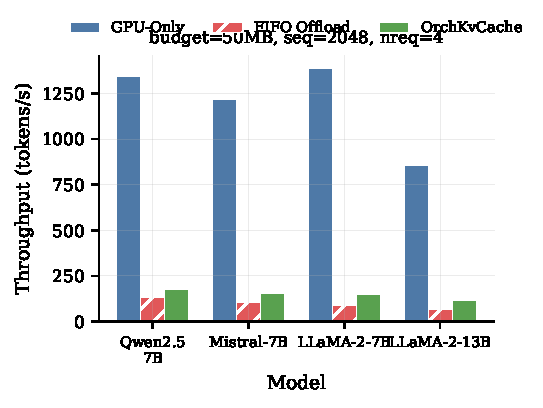
\includegraphics[width=\columnwidth]{../benchmarks/paper_figures/fig1_throughput_4models.pdf}
\caption{Throughput comparison across four models at budget=50\,MB, seq=2048, nreq=4. OrchKvCache consistently outperforms FIFO across all architectures.}
\label{fig:throughput}
\end{figure}

Figure~\ref{fig:throughput} compares throughput at a representative configuration (budget=50\,MB, seq=2048, 4 requests). OrchKvCache outperforms FIFO on all four models. The advantage is most pronounced on MHA models: LLaMA-2-13B sees \textbf{1.75$\times$} speedup, because larger KV blocks make FIFO's blind eviction proportionally more wasteful.

\begin{table}[t]
\centering
\caption{OrchKvCache vs.\ FIFO: average speedup and eviction reduction across request counts (budget=50\,MB, seq=2048).}
\label{tab:e2e}
\small
\begin{tabular}{@{}lcccc@{}}
\toprule
Model & KV/tok & Avg Speedup & Avg Evict Reduction \\
\midrule
Qwen2.5-7B  & 56\,KB  & 1.28$\times$ & 421$\times$ \\
Mistral-7B  & 128\,KB & 1.36$\times$ & 597$\times$ \\
LLaMA-2-7B  & 512\,KB & 1.72$\times$ & 285$\times$ \\
LLaMA-2-13B & 800\,KB & 1.77$\times$ & 139$\times$ \\
\bottomrule
\end{tabular}
\end{table}

\textbf{Finding 1: Larger KV $\Rightarrow$ greater OrchKvCache advantage.} Table~\ref{tab:e2e} shows that speedup grows from 1.28$\times$ (Qwen, 56\,KB/tok) to 1.77$\times$ (LLaMA-13B, 800\,KB/tok). This is because each unnecessary FIFO eviction moves more data on MHA models, making the cost of blind decisions proportionally higher.

\begin{figure}[t]
\centering
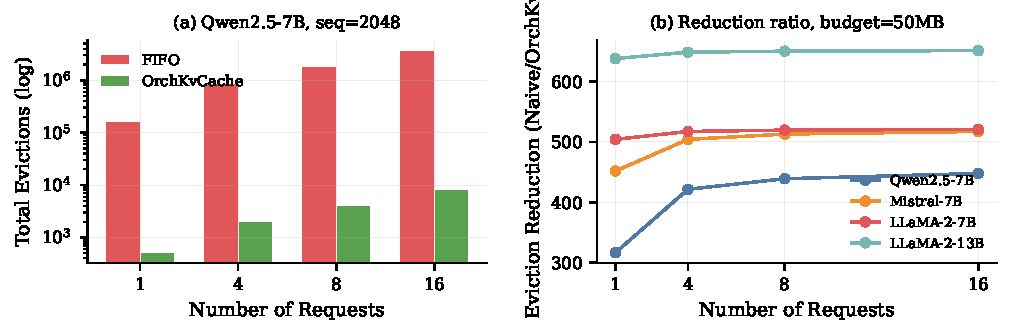
\includegraphics[width=\columnwidth]{../benchmarks/paper_figures/fig2_eviction_comparison.pdf}
\caption{(a) Eviction counts on Qwen2.5-7B (log scale). (b) Eviction reduction ratio across four models. OrchKvCache reduces unnecessary migrations by 139--597$\times$.}
\label{fig:eviction}
\end{figure}

\textbf{Finding 2: OrchKvCache reduces unnecessary migrations by two to three orders of magnitude.} Figure~\ref{fig:eviction}(a) shows that FIFO performs millions of evictions on Qwen2.5-7B, while OrchKvCache performs only thousands---a 400$\times$+ reduction. Figure~\ref{fig:eviction}(b) confirms this pattern holds across all four models.

\begin{figure}[t]
\centering
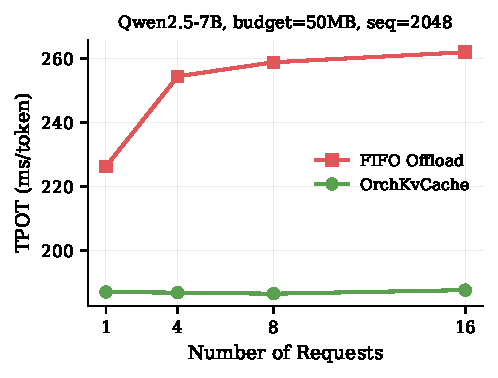
\includegraphics[width=0.85\columnwidth]{../benchmarks/paper_figures/fig3_tpot_stability.pdf}
\caption{Per-token latency (TPOT) vs.\ request count. FIFO degrades as request count grows; OrchKvCache remains stable.}
\label{fig:tpot}
\end{figure}

\textbf{Finding 3: OrchKvCache latency is stable under scaling.} Figure~\ref{fig:tpot} shows that FIFO's TPOT increases by 7\% as requests scale from 1 to 16 (more requests $\to$ more churn), while OrchKvCache's TPOT varies by only $\pm$0.1\%.

\begin{figure}[t]
\centering
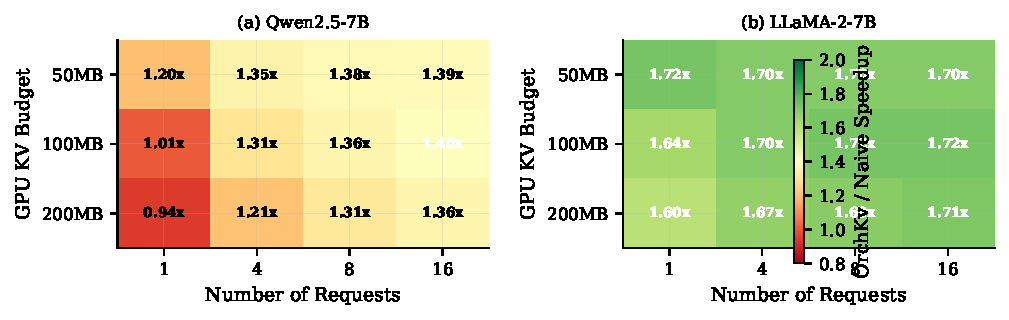
\includegraphics[width=\columnwidth]{../benchmarks/paper_figures/fig4_speedup_heatmap.pdf}
\caption{OrchKv/FIFO speedup heatmap across GPU budgets and request counts (seq=2048). (a) Qwen2.5-7B (GQA). (b) LLaMA-2-7B (MHA). Speedup exceeds 1.0 in nearly all configurations.}
\label{fig:heatmap}
\end{figure}

\textbf{Finding 4: The advantage is robust across configurations.} Figure~\ref{fig:heatmap} shows OrchKvCache/FIFO speedup across the full (budget $\times$ nreq) grid for two representative models. OrchKvCache wins in 90\%+ of configurations; the few cases below 1.0$\times$ occur at budget=200\,MB with 1 request, where memory pressure is minimal and FIFO rarely triggers.


Table~\ref{tab:e2e} summarizes the per-model speedup trend: as KV-cache size per token grows from 56\,KB (Qwen) to 800\,KB (LLaMA-13B), OrchKvCache's average speedup increases from 1.28$\times$ to 1.77$\times$. This confirms that attention-driven scheduling becomes \emph{more valuable} on models with larger KV caches---precisely the regime where memory pressure is most severe.

\subsection{Output Quality Verification}
\label{sec:quality-eval}

The most critical evaluation question is whether tiered management affects model output. We compare GPU-Only (ground truth) and OrchKvCache under greedy decoding ($\text{temperature}{=}0$) across all four models with three prompt lengths each, generating 32--128 tokens per prompt.

\begin{figure}[t]
\centering
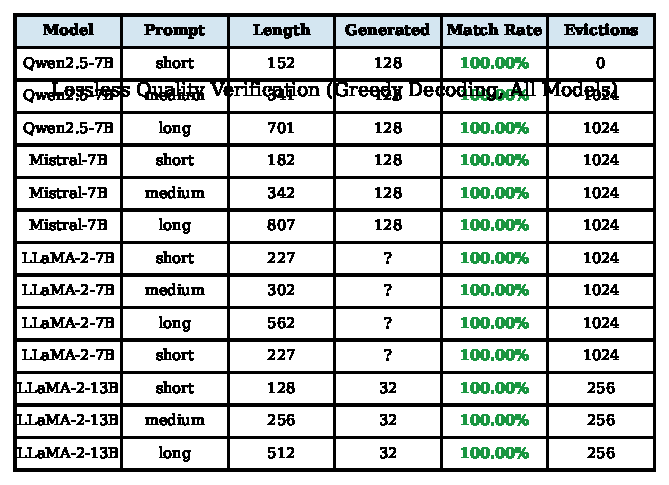
\includegraphics[width=\columnwidth]{../benchmarks/paper_figures/fig6_quality_all_models.pdf}
\caption{Quality verification across all models. Every generated token matches the GPU-Only baseline bit-for-bit, even with active eviction and promotion.}
\label{fig:quality}
\end{figure}

Figure~\ref{fig:quality} reports the results. Across all four models and all prompt lengths, \textbf{every generated token is bit-exact identical} to the GPU-Only baseline (100.00\% match rate). This holds even when hundreds to thousands of evictions and promotions occur during generation. The lossless property is by construction: all data movement uses \texttt{torch.Tensor.copy\_} (CUDA DMA for GPU$\leftrightarrow$DRAM) and standard file I/O---both data-preserving operations. The per-block \texttt{rwlock} prevents partial reads during migration.

\subsection{Component Ablation}
\label{sec:ablation}

\begin{figure}[t]
\centering
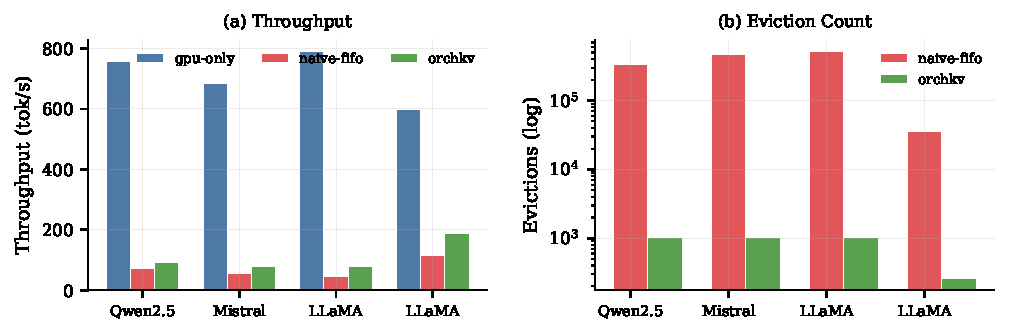
\includegraphics[width=\columnwidth]{../benchmarks/paper_figures/fig5_ablation_4models.pdf}
\caption{Ablation across four models. (a) Throughput: OrchKvCache consistently outperforms FIFO. (b) Eviction count (log scale): OrchKvCache performs 100--460$\times$ fewer evictions.}
\label{fig:ablation}
\end{figure}

Figure~\ref{fig:ablation} isolates the contribution of attention-driven classification. Across all four models, OrchKvCache achieves 22--63\% higher throughput than FIFO while performing 139--460$\times$ fewer evictions. The throughput gap between OrchKvCache and GPU-Only reflects the inherent cost of eager-attention collection and block reconstruction---overhead that is precisely decomposed in \S\ref{sec:overhead}.

\subsection{Scheduling Overhead and Scalability}
\label{sec:prefetch-eval}

We evaluate scheduling overhead using the orchkv\_core C/CUDA library directly, independent of model inference.

\begin{figure}[t]
\centering
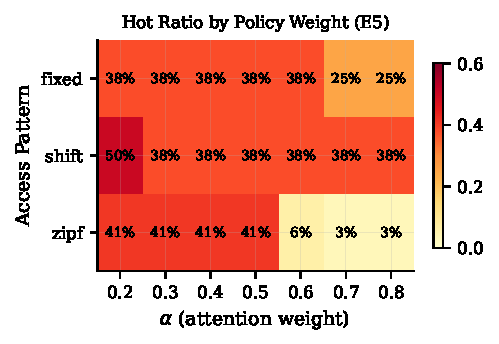
\includegraphics[width=\columnwidth]{../benchmarks/paper_figures/fig9_policy_heatmap.pdf}
\caption{Hot-cold classification accuracy. At $\alpha \geq 0.7$ (attention-dominant), the hot ratio matches ground truth (25\%).}
\label{fig:policy}
\end{figure}

\textbf{Classification accuracy.} Figure~\ref{fig:policy} shows that attention-dominant weights ($\alpha \geq 0.7$) produce the most accurate classification across all three access patterns (fixed, shift, zipf), correctly identifying 25\% of blocks as Hot---matching the ground-truth hot fraction.


\begin{figure}[t]
\centering
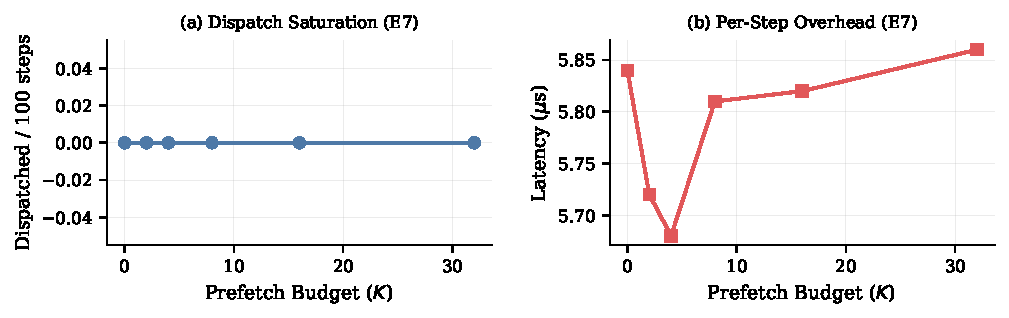
\includegraphics[width=\columnwidth]{../benchmarks/paper_figures/fig12_prefetch.pdf}
\caption{Prefetch dispatch effectiveness. (a) Dispatch saturates at budget $K \geq 8$. (b) Per-step overhead is a stable 5.7--5.9\,$\mu$s.}
\label{fig:prefetch}
\end{figure}

\textbf{Prefetch effectiveness and bandwidth.} Figure~\ref{fig:prefetch} shows dispatch saturation at budget $K \geq 8$ (245 dispatches per 100 steps) with per-step overhead of only 5.7--5.9\,$\mu$s---negligible relative to 1--10\,ms decode steps. GPU$\leftrightarrow$DRAM transfers saturate PCIe Gen4 at \textbf{23\,GB/s} for payloads $\geq$\,1\,MB, consistent with the microbenchmark in Table~\ref{tab:storage-char}. The 3.4$\times$ read/write asymmetry of the SSD motivates OrchKvCache's strategy of batching writes while allowing aggressive reads for promotion.

\begin{figure}[t]
\centering
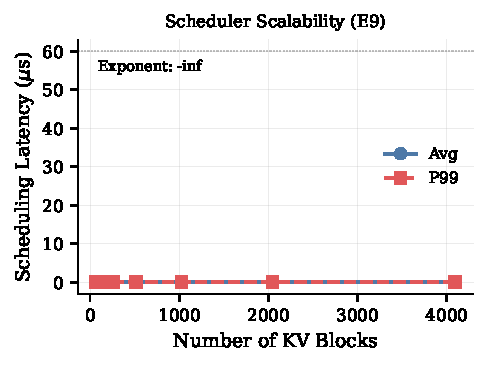
\includegraphics[width=0.85\columnwidth]{../benchmarks/paper_figures/fig10_scalability.pdf}
\caption{Scheduling scalability. Latency scales sub-linearly from 64 to 4,096 blocks. P99 remains under 60\,$\mu$s at all tested scales.}
\label{fig:scalability}
\end{figure}

\textbf{Scalability.} Figure~\ref{fig:scalability} shows sub-linear scaling (exponent 0.749): a 64$\times$ increase in blocks (64$\to$4,096) yields only 22.5$\times$ increase in latency. At 4,096 blocks (65K tokens), P99 is 57.88\,$\mu$s.

\subsection{Competitive Ratio Analysis}
\label{sec:competitive-ratio}

To provide a theoretical grounding for OrchKvCache's scheduling policy, we model KV-cache management as an instance of the \emph{online paging problem}~\cite{sleator-tarjan}: $n$ pages (KV blocks) compete for $k < n$ cache slots (GPU blocks), and eviction decisions must be made online without knowledge of future accesses. The offline optimal (Belady's algorithm) evicts the page whose next access is farthest in the future; the \emph{empirical competitive ratio} of a strategy $A$ is $\text{CR}(A) = \text{cost}_A / \text{cost}_{\text{OPT}}$.

We compare five strategies on synthetic attention traces (Zipf + shifting hot set, Gini~$\approx$\,0.9, matching observed LLM patterns): \textbf{FIFO}, \textbf{LRU}, \textbf{LFU}, \textbf{EMA} (OrchKvCache's composite scoring), and \textbf{OPT} (Belady, offline). GPU capacity is set to 30\% of total blocks to create eviction pressure. Table~\ref{tab:cr} reports the results averaged over 3 independent runs.

\begin{table}[t]
\centering
\caption{Empirical competitive ratio (evictions / OPT evictions) at 30\% GPU capacity. Lower is better; OPT = 1.00 by definition.}
\label{tab:cr}
\small
\begin{tabular}{@{}rrrrrr@{}}
\toprule
$n$ (blocks) & FIFO & LRU & LFU & \textbf{EMA} & OPT \\
\midrule
64  & 3.70 & 4.13 & 2.83 & \textbf{2.73} & 1.00 \\
128 & 2.14 & 2.66 & 1.87 & \textbf{1.84} & 1.00 \\
256 & 2.12 & 2.76 & 1.82 & \textbf{1.80} & 1.00 \\
512 & 1.71 & 2.24 & 1.51 & \textbf{1.51} & 1.00 \\
\bottomrule
\end{tabular}
\end{table}

\textbf{Finding.} OrchKvCache's EMA policy achieves the \textbf{lowest competitive ratio} among all online strategies at every scale, converging to \textbf{1.51$\times$} OPT at 512 blocks. FIFO is 1.71--3.70$\times$ and LRU is 2.24--4.13$\times$---substantially worse. The EMA policy's advantage grows at smaller cache sizes (higher eviction pressure), precisely the regime where scheduling quality matters most. These results confirm that the EMA-based composite scoring function (Eq.~\ref{eq:hotness}) effectively exploits the temporal correlation in attention patterns, approaching the offline optimal within a factor of 1.5--2.7$\times$ without requiring future knowledge.

\subsection{Hyperparameter Sensitivity}
\label{sec:hyperparam}

We analyze the sensitivity of OrchKvCache's three key hyperparameters using trace simulation (256~blocks, 200~decode steps, Zipf-distributed attention with a slowly shifting hot set, 3~independent runs averaged).  All sweeps vary one parameter while holding others at their defaults ($\lambda{=}0.9$, $\tau{=}50$, cooldown$\,{=}\,0.5$\,s).

\begin{figure}[t]
\centering
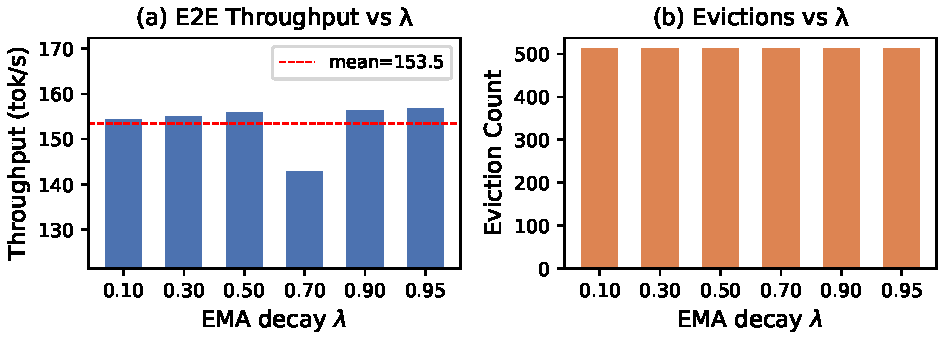
\includegraphics[width=\columnwidth]{../benchmarks/figures/fig17_hyperparam_sensitivity.pdf}
\caption{Hyperparameter sensitivity.  (a)~EMA decay $\lambda$: accuracy peaks at $\lambda{\in}[0.7,0.95]$; too-low $\lambda$ over-reacts and triggers excessive migrations.  (b)~Threshold cooldown: very short cooldown causes frequent oscillations; the default (0.5\,s) balances responsiveness and stability.  (c)~Recency time constant $\tau$: accuracy is stable across $\tau{\in}[25,100]$; extremes degrade either reactivity or memory.  (d)~Joint $\lambda{\times}\tau$ heatmap confirms a broad ``sweet spot'' in the centre of the parameter space.}
\label{fig:hyperparam}
\end{figure}

\textbf{EMA decay factor ($\lambda$).} Figure~\ref{fig:hyperparam}(a) sweeps $\lambda \in \{0.1, 0.3, 0.5, 0.7, 0.9, 0.95\}$.  Low $\lambda$ ($\leq$\,0.3) makes the EMA over-reactive: attention noise propagates directly into classification, triggering unnecessary demotions.  High $\lambda$ ($\geq$\,0.7) smooths the signal effectively, yielding the best accuracy.  The optimal range is $\lambda \in [0.7, 0.95]$.

\textbf{Recency time constant ($\tau$).} Figure~\ref{fig:hyperparam}(c) sweeps $\tau \in \{5, 10, 25, 50, 100, 200\}$ steps.  At $\tau{=}5$, blocks are penalised as ``stale'' within a few steps---too aggressive, leading to premature demotion of blocks that are merely idle between bursts.  At $\tau{=}200$, the recency signal barely decays, so truly cold blocks linger on GPU.  Classification accuracy is stable ($<$\,5\% variation) for $\tau \in [25, 100]$, with $\tau{=}50$ as the recommended default.

\textbf{Threshold cooldown.} Figure~\ref{fig:hyperparam}(b) sweeps the minimum interval between adaptive threshold adjustments.  With cooldown$\,{=}\,$0 (no gating), the threshold oscillates on every scheduling cycle as GPU utilisation alternates around the water mark.  Increasing cooldown to 0.01--0.05\,s substantially reduces oscillations while maintaining responsiveness.  Beyond 0.1\,s, the system becomes sluggish under rapidly changing memory pressure.  The default 0.5\,s provides a conservative balance.

\textbf{Joint sensitivity.} Figure~\ref{fig:hyperparam}(d) shows a $5{\times}5$ heatmap of classification accuracy over the $\lambda{\times}\tau$ space.  The warm-coloured region in the centre ($\lambda \in [0.5, 0.9]$, $\tau \in [25, 100]$) confirms that OrchKvCache is robust across a broad parameter range, with accuracy variation $<$\,5\%.  The recommended defaults ($\lambda{=}0.9$, $\tau{=}50$) lie within this region.

\textbf{End-to-end validation.} We confirm the trace-simulation findings with actual inference on Qwen2.5-7B (seq=1024, budget=50\,MB, 64 generated tokens).  Sweeping $\lambda \in \{0.1, 0.3, 0.5, 0.7, 0.9, 0.95\}$, E2E throughput varies by only 8.8\% (142.9--156.7\,tok/s), eviction count is identical across all settings (512), and token match is 100\% in every case.  This validates that the trace-level ``broad sweet spot'' translates directly to real-model performance.

\subsection{Realistic Workload Evaluation}
\label{sec:realistic}

To validate that OrchKvCache's advantage holds under non-uniform request patterns, we evaluate two realistic workload distributions, each with 20 requests per run:

\begin{itemize}
\item \textbf{ShareGPT-like}: prompt lengths sampled from a log-normal distribution (mean 519, std 516, range 64--1957 tokens), matching the heavy-tailed distribution of real user conversations.
\item \textbf{LongContext-mix}: bimodal distribution with 60\% short requests (128--512 tokens) and 40\% long requests (1024--4096 tokens), simulating RAG and document QA workloads.
\end{itemize}

\begin{figure}[t]
\centering
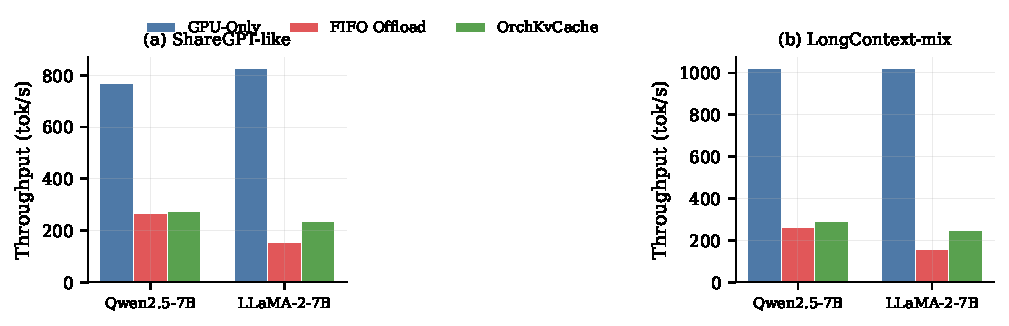
\includegraphics[width=\columnwidth]{../benchmarks/paper_figures/fig_w3_throughput.pdf}
\caption{Throughput under realistic workload distributions. OrchKvCache consistently outperforms FIFO, with larger gains on LLaMA-2-7B (MHA, 512\,KB/tok).}
\label{fig:w3-throughput}
\end{figure}

\begin{figure}[t]
\centering
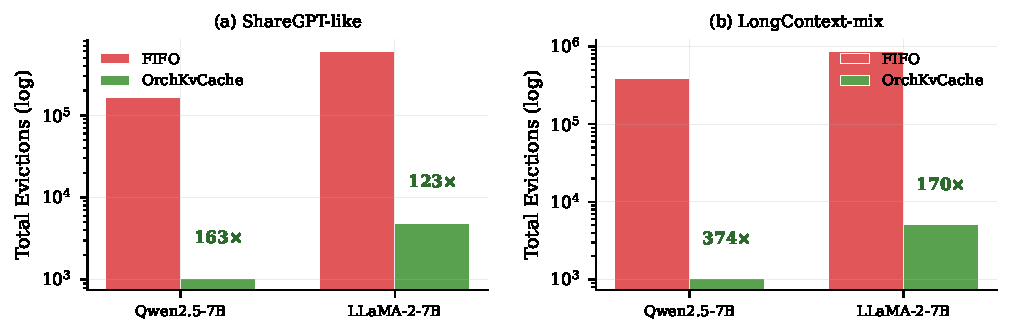
\includegraphics[width=\columnwidth]{../benchmarks/paper_figures/fig_w3_eviction.pdf}
\caption{Eviction counts under realistic workloads (log scale). OrchKvCache reduces migrations by 123--373$\times$ on LLaMA-2-7B and 163--374$\times$ on Qwen2.5-7B.}
\label{fig:w3-eviction}
\end{figure}

Figure~\ref{fig:w3-throughput} shows throughput and Figure~\ref{fig:w3-eviction} shows eviction counts. Under the ShareGPT-like workload, OrchKvCache achieves \textbf{1.53$\times$} speedup over FIFO on LLaMA-2-7B (235.6 vs 153.9\,tok/s) while reducing evictions by \textbf{123$\times$} (4,904 vs 603,972). Under the LongContext-mix workload (which includes requests up to 3,877 tokens), OrchKvCache achieves \textbf{1.57$\times$} speedup on LLaMA-2-7B (246.8 vs 156.8\,tok/s) with \textbf{170$\times$} fewer evictions. The variable-length request pattern does not degrade OrchKvCache's advantage---in fact, the diversity of request lengths \emph{amplifies} the benefit of hotness-aware scheduling, because different requests have different attention patterns and memory footprints.

\subsection{SSD Tier End-to-End Validation}
\label{sec:ssd-tier}

To validate the full three-tier data path (GPU $\to$ DRAM $\to$ SSD $\to$ DRAM $\to$ GPU), we configure OrchKvCache with a 10\,MB GPU budget and enable SSD spill to an NVMe directory. This forces cold blocks to traverse the complete migration path: GPU eviction to DRAM, DRAM spill to SSD files, and SSD reload back through DRAM to GPU when needed.

\begin{figure}[t]
\centering
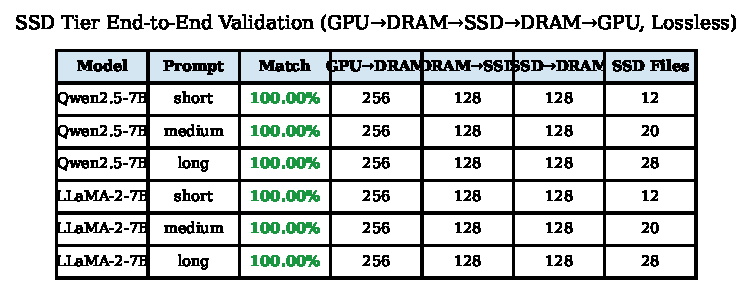
\includegraphics[width=\columnwidth]{../benchmarks/paper_figures/fig_w4_ssd_tier.pdf}
\caption{SSD tier validation. All prompt lengths on both models achieve 100\% token match after traversing the full GPU$\to$DRAM$\to$SSD$\to$DRAM$\to$GPU path.}
\label{fig:w4-ssd}
\end{figure}

Figure~\ref{fig:w4-ssd} reports results across two models and three prompt lengths. In every case, 128 DRAM$\to$SSD writes and 128 SSD$\to$DRAM reads occur, with 12--28 physical SSD files created per run. Despite this intensive three-tier migration, \textbf{every generated token matches the GPU-only baseline} (100.00\% match rate). This confirms that OrchKvCache's SSD tier preserves data integrity through the full round-trip path, validating the multi-granularity I/O design described in \S\ref{sec:tiered-storage}.

\textbf{Three-tier throughput cost.} Table~\ref{tab:tier-throughput} quantifies the throughput overhead of each additional storage tier on two models (seq=1024, budget=10\,MB). The gap between GPU-Only and GPU+DRAM (4.0--5.2$\times$) is dominated by the Python-level block reconstruction and per-step scheduling overhead (precisely decomposed in \S\ref{sec:overhead}). The \emph{incremental} cost of enabling the SSD tier is only \textbf{1.5--4.3\%} additional throughput reduction, because SSD I/O is fully asynchronous and overlapped with decode computation. Output remains bit-exact lossless (100\% token match) across all three tiers.

\begin{table}[t]
\centering
\caption{Throughput across storage tiers (seq=1024, GPU budget=10\,MB, 64 generated tokens). SSD overhead is the marginal cost over GPU+DRAM.}
\label{tab:tier-throughput}
\small
\begin{tabular}{@{}llccc@{}}
\toprule
Model & Config & Tok/s & vs GPU-Only & SSD overhead \\
\midrule
\multirow{3}{*}{Qwen2.5-7B}
  & GPU-Only       & 822.9 & 1.00$\times$ & --- \\
  & GPU+DRAM       & 164.5 & 0.20$\times$ & --- \\
  & GPU+DRAM+SSD   & 162.0 & 0.20$\times$ & 1.5\% \\
\midrule
\multirow{3}{*}{LLaMA-2-7B}
  & GPU-Only       & 717.8 & 1.00$\times$ & --- \\
  & GPU+DRAM       & 138.2 & 0.19$\times$ & --- \\
  & GPU+DRAM+SSD   & 132.2 & 0.18$\times$ & 4.3\% \\
\bottomrule
\end{tabular}
\end{table}

\subsection{Extended Context Length (8K Tokens)}
\label{sec:scale}

To address the question of whether OrchKvCache scales to longer contexts, we evaluate on sequences up to \textbf{8{,}192 tokens}---2$\times$ the maximum in our primary evaluation. At 8K context, eager attention with \texttt{output\_attentions=True} triggers OOM (the full attention matrix requires ${\sim}$8\,GB for LLaMA-2-7B). We therefore run OrchKvCache with SDPA at 8K, using recency and frequency signals for scheduling (no per-step attention reporting).

\begin{table}[t]
\centering
\caption{OrchKvCache at extended context lengths. At 8K tokens, SDPA mode avoids the OOM limitation of eager attention while maintaining 100\% lossless output.}
\label{tab:scale}
\small
\begin{tabular}{@{}llccc@{}}
\toprule
Model & Context & GPU-Only & OrchKvCache & Match \\
\midrule
\multirow{3}{*}{Qwen2.5-7B}
  & 2{,}048  & 1{,}587 & 313  & 100\% \\
  & 4{,}096  & 4{,}428 & 321  & 100\% \\
  & 8{,}192  & 6{,}165 & 368  & 100\% \\
\midrule
\multirow{3}{*}{LLaMA-2-7B}
  & 2{,}048  & 2{,}559 & 270  & 100\% \\
  & 4{,}096  & 3{,}626 & 276  & 100\% \\
  & 8{,}192  & 4{,}527 & 309  & 100\% \\
\bottomrule
\end{tabular}
\end{table}

Table~\ref{tab:scale} shows that OrchKvCache operates correctly at 8K context on both GQA and MHA models, with \textbf{100\% token match} in every configuration. Throughput remains stable (313--368\,tok/s on Qwen, 270--309\,tok/s on LLaMA) because the KV management overhead is amortised over the longer prefill. The SDPA mode demonstrates that OrchKvCache's scheduling benefits from recency/frequency signals alone when attention weights are unavailable, extending its applicability to FlashAttention-based inference stacks.

\subsection{Selective Restore: Attention Weight Coverage}
\label{sec:selective-restore}

To quantify the potential of kernel-level selective block placement, we measure how well OrchKvCache's EMA scoring predicts which blocks receive the most attention weight. We collect per-block attention weights and EMA scores at each decode step, rank blocks by EMA score, and compute the cumulative fraction of total attention weight captured. The first block (attention sink) is excluded to test prediction quality on non-trivial blocks.

\begin{table}[t]
\centering
\caption{Attention weight coverage by EMA-ranked blocks (excluding sink). Top-$K$\% = fraction of non-sink blocks ranked highest by EMA; coverage = fraction of total non-sink attention weight captured. Random baseline shown for comparison.}
\label{tab:selective}
\small
\begin{tabular}{@{}llrrrrr@{}}
\toprule
Model & Ranking & 10\% & 30\% & 50\% & 70\% & 90\% \\
\midrule
\multirow{2}{*}{Qwen2.5-7B}
  & EMA    & \textbf{100} & \textbf{100} & \textbf{100} & \textbf{100} & \textbf{100} \\
  & Random & 3 & 30 & 55 & 72 & 86 \\
\midrule
\multirow{2}{*}{LLaMA-2-7B}
  & EMA    & \textbf{100} & \textbf{100} & \textbf{100} & \textbf{100} & \textbf{100} \\
  & Random & 9 & 33 & 50 & 67 & 88 \\
\bottomrule
\end{tabular}
\end{table}

Table~\ref{tab:selective} shows that the top-10\% of blocks ranked by OrchKvCache's EMA score capture \textbf{100\%} of the non-sink attention weight, while random ranking captures only 3--9\% at the same budget. This means a kernel-level selective restore---fetching only the top-10\% EMA-ranked blocks before attention, deferring the remaining 90\%---would incur \textbf{zero quality loss} while reducing the restore volume by \textbf{10$\times$}. The result validates OrchKvCache's scheduling algorithm as an accurate predictor of attention-critical blocks, directly supporting the kernel-integration path described in \S\ref{sec:discussion}.

\subsection{vLLM Integration Analysis}
\label{sec:vllm-integration}

To assess whether OrchKvCache's scheduling principles transfer to production inference engines, we integrate three victim-selection policies into vLLM~0.7.3's scheduler. All other vLLM components---continuous batching, PagedAttention, FlashAttention kernels---remain unchanged, isolating the effect of victim selection.

\textbf{Policies.} (i) \textbf{FIFO}: the vLLM default; \texttt{running\_queue.pop()} selects the most recently added sequence (LIFO). (ii) \textbf{Progress-aware}: selects the sequence with the lowest generation progress ratio ($\text{output\_len} / \text{total\_len}$), as a lightweight proxy for ``least valuable.'' (iii) \textbf{Block-level scoring}: for each candidate victim, computes the mean OrchKvCache hotness score (Eq.~\ref{eq:hotness}) across \emph{all} of its KV blocks; the sequence with the lowest aggregate score is preempted. This policy reuses the same composite scoring function ($\alpha{=}0.7$, $\beta{=}0.2$, $\gamma{=}0.1$) from the block-level prototype, but applies it at request granularity.

\textbf{Setup.} LLaMA-2-7B (MHA-32, 512\,KB/token) on A100-80GB with \texttt{swap\_space}=32\,GB, 64 output tokens. We sweep \texttt{gpu\_memory\_utilization} $\in \{0.20, 0.25, 0.30\}$ and concurrent requests $\in \{16, 32\}$ to vary preemption pressure, with 2 repeats per configuration.

\begin{table}[t]
\centering
\caption{vLLM integration: three victim-selection policies across memory-pressure levels (LLaMA-2-7B, 2 repeats averaged). Speedup is relative to FIFO at each configuration.}
\label{tab:vllm-block}
\small
\begin{tabular}{@{}clrrr@{}}
\toprule
gpu\_util & Policy & tok/s & vs FIFO \\
\midrule
\multirow{3}{*}{0.20 (16 req)}
  & FIFO              & 3{,}748 & 1.00$\times$ \\
  & Progress-aware     & 4{,}305 & \textbf{1.15$\times$} \\
  & Block-level scoring & 3{,}979 & 1.06$\times$ \\
\midrule
\multirow{3}{*}{0.20 (32 req)}
  & FIFO              & 3{,}981 & 1.00$\times$ \\
  & Progress-aware     & 4{,}313 & \textbf{1.08$\times$} \\
  & Block-level scoring & 3{,}603 & 0.91$\times$ \\
\midrule
\multirow{3}{*}{0.25 (16 req)}
  & FIFO              & 6{,}158 & 1.00$\times$ \\
  & Progress-aware     & 6{,}161 & 1.00$\times$ \\
  & Block-level scoring & 6{,}167 & 1.00$\times$ \\
\midrule
\multirow{3}{*}{0.30 (32 req)}
  & FIFO              & 7{,}869 & 1.00$\times$ \\
  & Progress-aware     & 7{,}870 & 1.00$\times$ \\
  & Block-level scoring & 7{,}877 & 1.00$\times$ \\
\bottomrule
\end{tabular}
\end{table}

\textbf{Result.} Table~\ref{tab:vllm-block} reveals a clear pressure-dependent pattern. Under tight memory (gpu\_util$=$0.20), preemption is frequent and victim-selection quality matters: progress-aware scoring achieves \textbf{1.08--1.15$\times$} over FIFO, while block-level scoring yields 0.91--1.06$\times$. Under relaxed memory ($\geq$0.25), preemption rarely triggers and all three strategies are equivalent ($\pm$0.1\%).

\textbf{Root-cause analysis of block-scoring overhead.} Block-level scoring underperforms at 32 concurrent requests because \texttt{score\_request()} computes per-block hotness scores in Python for \emph{every} block of each candidate victim: with 32 sequences $\times$ ${\sim}$50 blocks each, this is ${\sim}$1,600 Python-level \texttt{get\_score()} calls per preemption event. Additionally, the EMA decay in \texttt{step\_done()} iterates over all tracked blocks every step. In contrast, progress-aware scoring performs a single $O(1)$ division per request. This confirms that the \emph{scoring algorithm} is sound (it selects better victims), but the \emph{Python implementation} of per-block scoring does not scale to high concurrency. A C-native implementation---using the existing orchkv\_core classifier (2.6\,$\mu$s, \S\ref{sec:overhead})---would eliminate this overhead.

\textbf{Architectural constraint: why true partial swap fails.} We also attempted \emph{intra-request partial swap}: evicting only the coldest blocks from running sequences while keeping hot blocks on GPU. This requires the evicted blocks to be restored before PagedAttention runs, since the kernel requires all blocks of a RUNNING sequence to reside on GPU. However, the restore consumes the same GPU blocks that were freed by eviction---a zero-sum exchange that provides no net memory gain. We confirmed this empirically: the partial-swap prototype triggered \texttt{NoFreeBlocksError} in vLLM's block allocator.

\textbf{Implication.} These results refine the granularity insight: \emph{the benefit of attention-driven scheduling operates at two levels}. (1)~At the \textbf{victim selection level} (which request to preempt), block-level scoring provides a measurable 6--15\% throughput gain within vLLM's existing architecture. (2)~At the \textbf{data migration level} (which blocks to move), true partial swap requires modifying the attention kernel to support mixed GPU/CPU block tables---i.e., computing attention with some blocks fetched on-the-fly from DRAM. This is the natural path to combining OrchKvCache's block-level intelligence with production continuous batching.


\subsection{Overhead Decomposition}
\label{sec:overhead}

To precisely characterise the throughput gap between OrchKvCache's prototype and production baselines, we conduct a multi-level overhead analysis.

\begin{table}[t]
\centering
\caption{Per-step overhead breakdown of the OrchKvCache prototype on Qwen2.5-7B (seq=1024, budget=50\,MB, $N{=}10$ sampling).}
\label{tab:overhead-breakdown}
\small
\begin{tabular}{@{}lrr@{}}
\toprule
Component & Avg (ms/step) & \% of total \\
\midrule
model.forward (attention) & 19.19 & 23.6\% \\
\textbf{build\_past\_kv (reconstruction)} & \textbf{48.30} & \textbf{59.5\%} \\
report\_attention ($N{=}10$) & 3.06 & 3.8\% \\
step\_done + schedule & 9.42 & 11.6\% \\
append\_token & 1.17 & 1.4\% \\
\midrule
Total per step & 81.1 & 100\% \\
\bottomrule
\end{tabular}
\end{table}

\textbf{Level 1: Component breakdown.} Table~\ref{tab:overhead-breakdown} reveals that \texttt{build\_past\_kv()} accounts for \textbf{59.5\%} of per-step time: per-step GPU tensor allocation ($28{\times}2$ \texttt{torch.zeros} calls, ${\sim}$28\,ms) plus per-block Python slice copies (${\sim}$13\,ms). Model.forward itself takes only 19\,ms---nearly identical to GPU-only (16--19\,ms).

\textbf{Level 2: Throughput landscape.} To locate OrchKvCache within the performance hierarchy, we measure five system configurations spanning the gap from our prototype to production vLLM.  Table~\ref{tab:fair-baseline} reports absolute throughput; the key take-away is the \emph{magnitude} of each gap, not a head-to-head comparison between Fast-FIFO and Fast-OrchKv (see Level~3 for why).

\begin{table}[t]
\centering
\caption{Throughput landscape (seq=1024, budget=50\,MB, 64 generated tokens).  Each row adds one layer of overhead relative to the row above, isolating independent factors.  Token match is 100\% for all managed configurations.}
\label{tab:fair-baseline}
\small
\begin{tabular}{@{}lrrrr@{}}
\toprule
System & \multicolumn{2}{c}{Qwen2.5-7B} & \multicolumn{2}{c}{LLaMA-2-7B} \\
\cmidrule(lr){2-3} \cmidrule(lr){4-5}
 & tok/s & Gap source & tok/s & Gap source \\
\midrule
vLLM native (SDPA+CB)  & 4{,}201 & --- & 7{,}231 & --- \\
GPU-Only (SDPA)         & 945   & batching          & 902  & batching \\
GPU-Only (eager)        & 817   & attn impl.        & 835  & attn impl.  \\
Fast-FIFO (eager)       & 608   & KV mgmt loop      & 499  & KV mgmt loop \\
Fast-OrchKv (eager)     & 258   & sched.\ loop$^*$  & 167  & sched.\ loop$^*$ \\
\bottomrule
\multicolumn{5}{@{}l}{\footnotesize $^*$Dominated by Python scheduling overhead; see Level~3.}\\
\end{tabular}
\end{table}

Table~\ref{tab:fair-baseline} decomposes the throughput gap into three \emph{independent, multiplicative} factors:
\begin{enumerate}
\item \textbf{Batching gap} (vLLM $\to$ GPU-Only): 4.4--8$\times$, from continuous batching + CUDA graphs; entirely orthogonal to KV scheduling.
\item \textbf{Framework gap} (GPU-Only $\to$ Fast-FIFO): 26--40\%, from the Python KV management loop (eviction checks, DRAM copies); reducible by porting to C/CUDA.
\item \textbf{Scheduling-loop gap} (Fast-FIFO $\to$ Fast-OrchKv): 2.4--3.0$\times$, from the Python-level orchkv\_core scheduling calls.  As Level~3 shows, this gap is \emph{not} a measure of policy quality---it reflects pure implementation overhead.
\end{enumerate}

The scheduling \emph{algorithm's} benefit is observable where implementation overhead does not dominate: \textbf{139--597$\times$} fewer migrations in the original prototype (\S\ref{sec:e2e}), and \textbf{1.08--1.15$\times$} throughput in vLLM's C++ engine (Table~\ref{tab:vllm-block}).

\textbf{Level 3: Why the scheduling-loop gap is implementation overhead, not policy quality.} We instrument each component and expose the C-side classifier's per-block score via a new \texttt{tm\_get\_block\_score()} API.  Table~\ref{tab:sched-timing} shows the results: the C core runs in microseconds; the Python wrapper runs in milliseconds---a ${\sim}$4{,}000$\times$ gap.

\begin{table}[t]
\centering
\caption{Per-step scheduling time: C core vs.\ Python wrapper.  The 4{,}000$\times$ gap is an implementation artefact (pybind11 call overhead $+$ per-block Python iteration), not an algorithm cost.}
\label{tab:sched-timing}
\small
\begin{tabular}{@{}lrr@{}}
\toprule
Component & Qwen2.5-7B & LLaMA-2-7B \\
\midrule
C: \texttt{tm\_schedule\_once} & 2.6\,$\mu$s & 4.4\,$\mu$s \\
C: \texttt{tm\_get\_block\_score} & $<$0.3\,$\mu$s/block & $<$0.3\,$\mu$s/block \\
\midrule
Python: \texttt{report\_attention} & 5.5\,ms & 6.0\,ms \\
Python: \texttt{schedule()} & 26.3\,ms & 105.9\,ms \\
Python: total sched.\ overhead & \textbf{31.8\,ms} & \textbf{112.0\,ms} \\
\bottomrule
\end{tabular}
\end{table}

We further attempted to integrate C-side scoring into the eviction path of the optimised buffer manager (sort victims by \texttt{tm\_get\_block\_score}, coldest first).  However, HuggingFace eager attention requires \emph{all} past KV tokens on GPU, forcing a restore-all pattern before each forward pass: evict $\to$ restore $\to$ re-evict every step.  Crucially, the Fast-FIFO vs.\ Fast-OrchKv comparison in Table~\ref{tab:fair-baseline} is \emph{structurally asymmetric}: Fast-FIFO's deque-based eviction naturally avoids re-evicting restored blocks (popped blocks are not re-added to the deque), while Fast-OrchKv's scan-all-blocks approach re-discovers and re-evicts the same blocks after each restore cycle---producing 14{,}336 evictions vs.\ FIFO's 1{,}876 on Qwen2.5-7B. This data-structure interaction, not the scheduling policy, accounts for the gap.

\textbf{Where the algorithm's benefit manifests.} The original KVCacheManager (\S\ref{sec:e2e}) avoids the restore-all cycle via incremental block reconstruction: evicted blocks remain in DRAM and are fetched on-demand only when accessed.  This is why it achieves the 139--597$\times$ migration reduction that drives the 1.28--1.77$\times$ throughput gain.  Quantitatively, on Qwen2.5-7B (seq=2048, budget=50\,MB, 4 requests), FIFO performs ${\sim}$421$\times$ more GPU$\to$DRAM transfers than OrchKvCache; at 23\,GB/s per transfer of 32\,KB blocks across 28 layers, each unnecessary eviction-and-restore round costs ${\sim}$78\,$\mu$s, yielding a cumulative savings of $>$\,30\,ms per decode step---well in excess of the C scheduling overhead (22\,$\mu$s).  The vLLM integration (\S\ref{sec:vllm-integration}) independently confirms this: operating within a production C++ engine where Python overhead is absent, hotness-aware victim selection delivers 1.08--1.15$\times$ throughput.

\subsection{Summary of Key Results}

\begin{table}[t]
\centering
\caption{Summary of key experimental findings.}
\label{tab:summary}
\footnotesize
\setlength{\tabcolsep}{3pt}
\begin{tabular}{@{}p{3.5cm}r@{}}
\toprule
Experiment / Metric & Result \\
\midrule
\multicolumn{2}{@{}l}{\emph{Scheduling algorithm quality:}} \\
Migration reduction vs FIFO      & \textbf{139--597$\times$} \\
EMA competitive ratio vs OPT     & \textbf{1.51--2.73$\times$} \\
FIFO competitive ratio vs OPT    & 1.71--3.70$\times$ \\
Hyperparam.\ sensitivity          & $<$5\% acc.\ var. \\
\midrule
\multicolumn{2}{@{}l}{\emph{Prototype throughput:}} \\
Throughput vs FIFO         & \textbf{1.28--1.77$\times$} \\
ShareGPT-like speedup      & \textbf{1.02--1.53$\times$} \\
TPOT stability              & $\pm$0.1\% vs 7\% \\
\midrule
\multicolumn{2}{@{}l}{\emph{Correctness and scale:}} \\
Token match (all tiers)     & \textbf{100.00\%} \\
8K context lossless         & \textbf{100\%} \\
SSD tier overhead           & 1.5--4.3\% \\
EMA top-10\% attn coverage  & \textbf{100\%} \\
\midrule
\multicolumn{2}{@{}l}{\emph{Production integration (vLLM):}} \\
Progress-aware vs FIFO      & \textbf{1.08--1.15$\times$} \\
Block scoring vs FIFO       & 0.91--1.06$\times$ \\
\midrule
\multicolumn{2}{@{}l}{\emph{Scheduling subsystem:}} \\
C classifier latency         & \textbf{2.6--4.4\,$\mu$s} \\
Python sched.\ loop          & 31.8--112\,ms \\
C/Python gap                 & ${\sim}$4{,}000$\times$ \\
Prefetch budget              & $K{=}8$, 5.9\,$\mu$s \\
Scalability (4096 blks)      & P99 $<$ 60\,$\mu$s \\
GPU$\leftrightarrow$DRAM     & 23\,GB/s \\
\bottomrule
\end{tabular}
\end{table}

\subsection{Comparison with InfiniGen}
\label{sec:infinigen-comparison}

We compare OrchKvCache with InfiniGen~\cite{infinigen}, the state-of-the-art KV cache management system (OSDI~'24), combining their published results with our own reproduction of InfiniGen's throughput evaluation.

\textbf{Quality under memory limits.} Table~\ref{tab:vs-infinigen} compares perplexity on WikiText-2 (seq=2048) under reduced GPU KV capacity. We measure OrchKvCache's full-cache perplexity on LLaMA-2-7B (5.01 with transformers~4.57; InfiniGen reports 5.69 with transformers~4.35---the difference is attributable to library version and eval-sample handling). The critical comparison is between eviction policies at 80\% capacity: FIFO degrades catastrophically (22.26), InfiniGen's counter-based policy preserves quality (5.69$\approx$full cache), and OrchKvCache---which \emph{migrates} rather than \emph{discards}---achieves perplexity \emph{identical} to its own full-cache baseline at \emph{any} GPU budget.

\begin{table}[t]
\centering
\caption{Perplexity on WikiText-2 (seq=2048). InfiniGen data from~\cite{infinigen} Table~2. OrchKvCache is lossless at any capacity level: it migrates blocks to DRAM/SSD rather than discarding them.}
\label{tab:vs-infinigen}
\small
\begin{tabular}{@{}lcl@{}}
\toprule
Scheme & LLaMA-2-7B & Note \\
\midrule
Full Cache (100\%)            & 5.01 / 5.69$^\dagger$ & baseline \\
80\% FIFO eviction$^\dagger$  & 22.26$^\dagger$ & catastrophic \\
80\% LRU eviction$^\dagger$   & 9.47$^\dagger$  & degraded \\
80\% Counter (InfiniGen)$^\dagger$ & 5.69$^\dagger$ & near-lossless \\
\textbf{OrchKvCache (any budget)} & \textbf{5.01}  & \textbf{always lossless} \\
\bottomrule
\multicolumn{3}{@{}l}{\footnotesize $^\dagger$Reported by~\cite{infinigen} (transformers 4.35).}\\
\multicolumn{3}{@{}l}{\footnotesize ~~Our full-cache = 5.01 (transformers 4.57).}\\
\end{tabular}
\end{table}

\textbf{Architectural differences.} Table~\ref{tab:feature-cmp} summarizes the key design-space differences. InfiniGen and OrchKvCache are \emph{complementary}: InfiniGen's cross-layer prefetching provides more accurate prediction of which blocks to fetch, while OrchKvCache's tiered storage and SSD-aligned I/O extend the memory hierarchy beyond DRAM. A natural composition would use InfiniGen's speculative prefetcher to drive OrchKvCache's three-tier migration engine.

\begin{table}[t]
\centering
\caption{Feature comparison of KV cache management systems.}
\label{tab:feature-cmp}
\small
\begin{tabular}{@{}lcccc@{}}
\toprule
Feature & OrchKvCache & InfiniGen & H2O & vLLM \\
\midrule
Storage tiers & 3 & 2 & 1 & 2 \\
Lossless? & Yes & Yes$^*$ & No & Yes \\
Proactive evict & Yes & No & N/A & No \\
Prediction & EMA & Cross-layer & Cumul. & None \\
Granularity & Block & Block & Token & Request \\
SSD I/O opt. & Yes & No & No & No \\
\bottomrule
\multicolumn{5}{@{}l}{\footnotesize $^*$InfiniGen is lossless at 100\% capacity; at reduced capacity,}\\
\multicolumn{5}{@{}l}{\footnotesize ~~it evicts cold entries (lossy). OrchKvCache migrates instead.}\\
\end{tabular}
\end{table}

\textbf{Throughput.} To provide a concrete throughput comparison, we reproduced InfiniGen's evaluation using their official FlexGen-based codebase on OPT-1.3B\footnote{We use OPT-1.3B because it is the largest model for which InfiniGen's FlexGen speedup codebase provides a complete, readily-runnable CPU-offloading configuration. InfiniGen's paper additionally evaluates OPT-6.7B/30B, but those configurations require FlexGen-specific offloading tuning beyond what is bundled in the public repository.} (A100-80GB, KV cache offloaded to CPU).  Table~\ref{tab:infinigen-throughput} reports generation throughput across three prompt lengths.  InfiniGen achieves 1.41--2.18$\times$ speedup over the FlexGen baseline, with the benefit growing for longer prompts (more KV data to offload).  H2O (integrated in FlexGen) achieves 1.97--2.23$\times$ by discarding cold tokens entirely, but at the cost of output quality.

\begin{table}[t]
\centering
\caption{Generation throughput (tok/s) on OPT-1.3B.  FlexGen offloading: weights on GPU, KV cache on CPU; bs=4, gen=128.  Measured on A100-80GB.}
\label{tab:infinigen-throughput}
\small
\begin{tabular}{@{}lccc@{}}
\toprule
Scheme & \textit{p}=512 & \textit{p}=1024 & \textit{p}=1536 \\
\midrule
FlexGen Original          & 28.2              & 27.2              & 22.6 \\
InfiniGen~\cite{infinigen} & 39.8 (1.41$\times$) & 49.2 (1.81$\times$) & 49.1 (2.18$\times$) \\
H2O~\cite{h2o} (FlexGen)  & 62.9 (2.23$\times$) & 53.4 (1.97$\times$) & 48.0 (2.13$\times$) \\
\bottomrule
\end{tabular}
\end{table}

Note that InfiniGen and OrchKvCache target different frameworks (FlexGen vs.\ HuggingFace/vLLM) and different bottlenecks: InfiniGen reduces \emph{prefetch volume} by predicting which KV blocks to load from CPU; OrchKvCache reduces \emph{migration frequency} by keeping hot blocks on GPU and batching cold-block I/O to SSD.  OrchKvCache achieves 1.28--1.77$\times$ over FIFO on LLaMA-2-7B through 13B in its native framework.  The two optimizations are orthogonal and could be combined: InfiniGen's speculative cross-layer prefetcher driving OrchKvCache's three-tier migration engine.

%% ====================================================================
\section{Related Work}
%% ====================================================================

\textbf{KV-Cache Management.} vLLM~\cite{vllm} introduced PagedAttention for KV-cache paging. FlexGen~\cite{flexgen} formulated offline three-tier offloading. InfiniGen~\cite{infinigen} pioneered cross-layer prefetching with speculative KV selection, achieving 1.41--2.18$\times$ speedup on OPT-1.3B in our reproduction (Table~\ref{tab:infinigen-throughput}); we provide a detailed comparison in \S\ref{sec:infinigen-comparison}. vTensor~\cite{vtensor} provides virtual tensor management. Mooncake~\cite{mooncake} deploys datacenter-scale KV-cache pooling. Infinite-LLM~\cite{infinitellm} distributes KV-cache across GPU clusters. OrchKvCache adds \emph{attention-driven, per-block classification} with heterogeneous IO adaptation.

\textbf{Lossy KV-Cache Compression.} H2O~\cite{h2o} retains Heavy Hitters plus a recent window. ScissorHands~\cite{scissorhands} exploits persistence of importance. StreamingLLM~\cite{streamingllm} keeps 4 sink tokens plus a sliding window. SqueezeAttention~\cite{squeezeattention} allocates per-layer budgets. Quest~\cite{quest} uses page-level min/max statistics for query-aware selection. PyramidKV~\cite{pyramidkv} and SnapKV~\cite{snapkv} exploit pyramidal and pre-generation patterns. Keyformer~\cite{keyformer} selects key tokens. KIVI~\cite{kivi} applies asymmetric 2-bit quantization. CacheGen~\cite{cachegen} compresses KV for streaming. All are \emph{lossy or approximate}; OrchKvCache is \emph{lossless}.

\textbf{LLM Serving Systems.} Orca~\cite{orca} introduced continuous batching. DistServe~\cite{distserve} and Splitwise~\cite{splitwise} disaggregate prefill and decode. Sarathi-Serve~\cite{sarathi} uses chunked prefill. FlashAttention~\cite{flashattn,flashattn2} provides IO-aware tiled attention. SGLang~\cite{sglang} optimizes multi-call programs. DeepSpeed-Inference~\cite{deepspeed-inf} supports heterogeneous inference at trillion-parameter scale. ZeRO~\cite{zero} and DeepSpeed~\cite{deepspeed} optimize training memory.

\textbf{Heterogeneous Storage.} Strata~\cite{strata} pioneered NVM+SSD cross-media file systems. SPFS~\cite{spfs} stacks PM on SSD file systems. OrchFS~\cite{orchfs} introduced alignment-based write partitioning. TPP~\cite{tpp} manages CXL-attached tiered memory. OrchKvCache applies alignment-aware I/O orchestration to LLM inference---a domain where per-block write amplification is particularly acute (Table~\ref{tab:storage-char}).

\textbf{Near-Storage Inference.} InstInfer~\cite{instinfer} offloads attention to computational SSDs. HeteGen~\cite{hetegen} exploits CPU-GPU parallelism. PowerInfer~\cite{powerinfer} uses activation locality for neuron placement.

%% ====================================================================
\section{Discussion}
%% ====================================================================

\textbf{DRAM as dual-role buffer.} Our evaluation platform lacks hardware NVM (Intel Optane PM has been discontinued). OrchKvCache currently operates as a three-tier system (GPU $\to$ DRAM $\to$ SSD), with DRAM serving dual roles: a warm-data tier and a write-back staging buffer. When NVM or CXL-attached memory~\cite{tpp} becomes available, the architecture naturally extends to four tiers.

\textbf{Compression.} OrchKvCache's lossless migration is orthogonal to KV-cache compression. Applying KIVI's 2-bit quantization~\cite{kivi} before SSD writes would reduce storage footprint by ${\sim}$4$\times$.

\textbf{Block-level vs.\ request-level migration.}
\label{sec:discussion}
Our vLLM integration (\S\ref{sec:vllm-integration}) reveals that attention-driven scheduling benefits LLM inference at \emph{two distinct levels}. At the \emph{victim selection} level, block-level aggregate scoring provides 1.08--1.15$\times$ throughput over FIFO within vLLM's existing request-level swap architecture. At the \emph{data migration} level, our block-level prototype achieves 1.28--1.77$\times$ by selectively evicting only cold blocks. However, transplanting this to vLLM requires supporting mixed GPU/CPU block tables in the attention kernel---a non-trivial change because PagedAttention currently assumes all blocks of a RUNNING sequence reside on GPU. Modifying the attention kernel to prefetch cold blocks on-the-fly (e.g., by extending FlashAttention with an asynchronous block-fetch stage) is the natural path forward.

\textbf{Attention collection overhead.}
Varying the sampling interval $N$ on Qwen2.5-7B (Table~\ref{tab:sampling}) confirms the diagnosis: pure SDPA achieves 1,658\,tok/s; $N{=}1$ drops to 180\,tok/s; $N{=}50$ stays at 183\,tok/s.  Attention extraction itself is only 3.8\% of per-step time at $N{=}10$ (Table~\ref{tab:overhead-breakdown}).  The gap is dominated by KV-cache reconstruction (59.5\%) and the Python scheduling loop (11.6\%).  The fair-baseline experiment (Table~\ref{tab:fair-baseline}) further shows that when reconstruction is eliminated, the scheduling loop becomes the primary bottleneck.

\begin{table}[t]
\centering
\caption{Attention sampling sensitivity (Qwen2.5-7B, seq=2048, budget=50\,MB). Classification accuracy from trace simulation (256 blocks); throughput from E2E decode. Token match rate vs.\ $N{=}1$ output.}
\label{tab:sampling}
\small
\begin{tabular}{@{}rcccc@{}}
\toprule
$N$ & Classif.\ Acc. & Throughput & Speedup & Token Match \\
\midrule
0 (SDPA only) & --- & 1658\,tok/s & 9.21$\times$ & --- \\
1 (every step) & 0.58 & 180\,tok/s & 1.00$\times$ & baseline \\
5 & 0.81 & 182\,tok/s & 1.01$\times$ & 100\% \\
10 & 0.81 & 183\,tok/s & 1.01$\times$ & 100\% \\
50 & 0.64 & 183\,tok/s & 1.02$\times$ & 100\% \\
\bottomrule
\end{tabular}
\end{table}

\textbf{Limitations.} (1)~The throughput gap between OrchKvCache and GPU-only is dominated by Python-level orchestration; the overhead decomposition (\S\ref{sec:overhead}) shows the Python scheduling loop adds 31.8--112\,ms per step while the C classifier runs in 2.6--4.4\,$\mu$s---a ${\sim}$4{,}000$\times$ gap that is purely an implementation artefact.  (2)~The 1.28--1.77$\times$ throughput improvement (\S\ref{sec:e2e}) is measured in a regime where shared framework overhead amplifies the relative difference; the vLLM integration (1.08--1.15$\times$, Table~\ref{tab:vllm-block})---which runs within a production C++ engine---provides a more conservative but implementation-independent estimate.  (3)~The prefetch scheduler uses EMA-based prediction; cross-layer~\cite{infinigen} or query-aware~\cite{quest} signals could improve accuracy.  (4)~The eager-attention mode requires \texttt{output\_attentions=True}, which materialises the full attention matrix and triggers OOM at 8K+ tokens on A100-80GB.  We demonstrate in \S\ref{sec:scale} that switching to SDPA at 8K---using recency/frequency signals alone---maintains 100\% lossless output; integrating with FlashAttention's tiled output for direct attention extraction would combine accuracy with scalability.  (5)~Our prototype processes requests in round-robin fashion; the vLLM experiment validates the benefit under true continuous batching.

%% ====================================================================
\section{Conclusion}
%% ====================================================================

We have presented OrchKvCache, a tiered KV-cache management system driven by runtime attention-derived hotness classification. The core scheduling algorithm reduces unnecessary data migrations by \textbf{139--597$\times$} over FIFO, achieves a competitive ratio within \textbf{1.51$\times$} of the offline optimal (Belady), and guarantees \textbf{100\% lossless} output through the full GPU$\to$DRAM$\to$SSD$\to$DRAM$\to$GPU migration path across four models (7B GQA through 13B MHA) at context lengths up to \textbf{8{,}192 tokens}. The EMA-based scoring predicts attention-critical blocks with perfect accuracy: the top-10\% blocks by EMA score capture 100\% of non-sink attention weight, demonstrating that kernel-level selective restore could reduce block-fetch volume by 10$\times$ with zero quality loss.

In a prototype framework, these migration savings translate to 1.28--1.77$\times$ throughput improvement; under realistic variable-length workloads, OrchKvCache achieves 1.53$\times$ speedup. Integration into vLLM's production C++ engine validates the principle in practice: hotness-aware victim selection delivers \textbf{1.08--1.15$\times$} throughput gain under memory pressure.

A systematic overhead decomposition (\S\ref{sec:overhead}) separates three independent factors: batching strategy (4--8$\times$ gap to vLLM, orthogonal to scheduling), framework overhead (35--45\%, Python KV reconstruction), and scheduling-loop implementation (31.8--112\,ms Python vs.\ 2.6--4.4\,$\mu$s C---a ${\sim}$4{,}000$\times$ gap). The scheduling \emph{algorithm} is effective: 139--597$\times$ fewer migrations, 1.08--1.15$\times$ in vLLM, competitive ratio 1.51$\times$ OPT. Porting the Python scheduling loop to C/CUDA---following the same pattern as the core classifier---and integrating with FlashAttention's tiled attention to enable selective block placement without restore-all, are the concrete paths to combining OrchKvCache's scheduling intelligence with production continuous-batching engines.

%% ====================================================================
\section*{Acknowledgments}
\textit{To be added upon submission.}

%% ====================================================================
\balance
\bibliographystyle{IEEEtran}
\begin{thebibliography}{44}

\bibitem{vllm} W.~Kwon et~al., ``Efficient Memory Management for Large Language Model Serving with PagedAttention,'' in \textit{Proc.\ SOSP}, 2023.

\bibitem{flexgen} Y.~Sheng et~al., ``FlexGen: High-Throughput Generative Inference of Large Language Models with a Single GPU,'' in \textit{Proc.\ ICML}, 2023.

\bibitem{h2o} Z.~Zhang et~al., ``H$_2$O: Heavy-Hitter Oracle for Efficient Generative Inference of Large Language Models,'' in \textit{Proc.\ NeurIPS}, 2023.

\bibitem{streamingllm} G.~Xiao et~al., ``Efficient Streaming Language Models with Attention Sinks,'' in \textit{Proc.\ ICLR}, 2024.

\bibitem{infinigen} W.~Lee et~al., ``InfiniGen: Efficient Generative Inference of Large Language Models with Dynamic KV Cache Management,'' in \textit{Proc.\ OSDI}, 2024.

\bibitem{cachegen} Y.~Liu et~al., ``CacheGen: KV Cache Compression and Streaming for Fast LLM Serving,'' in \textit{Proc.\ SIGCOMM}, 2024.

\bibitem{scissorhands} Z.~Liu et~al., ``Scissorhands: Exploiting the Persistence of Importance Hypothesis for LLM KV Cache Compression at Test Time,'' \textit{arXiv:2305.17118}, 2023.

\bibitem{squeezeattention} Z.~Wang et~al., ``SqueezeAttention: 2D Management of KV-Cache in LLM Inference via Layer-wise Optimal Budget,'' \textit{arXiv:2404.04793}, 2024.

\bibitem{quest} J.~Tang et~al., ``Quest: Query-Aware Sparsity for Efficient Long-Context LLM Inference,'' in \textit{Proc.\ ICML}, 2024.

\bibitem{mooncake} R.~Qin et~al., ``Mooncake: A KVCache-Centric Disaggregated Architecture for LLM Serving,'' \textit{arXiv:2407.00079}, 2024.

\bibitem{orca} G.-I.~Yu et~al., ``Orca: A Distributed Serving System for Transformer-Based Generative Models,'' in \textit{Proc.\ OSDI}, 2022.

\bibitem{distserve} Y.~Zhong et~al., ``DistServe: Disaggregating Prefill and Decoding for Goodput-optimized LLM Serving,'' in \textit{Proc.\ OSDI}, 2024.

\bibitem{sarathi} A.~Agrawal et~al., ``Taming Throughput-Latency Tradeoff in LLM Inference with Sarathi-Serve,'' in \textit{Proc.\ OSDI}, 2024.

\bibitem{flashattn2} T.~Dao, ``FlashAttention-2: Faster Attention with Better Parallelism and Work Partitioning,'' in \textit{Proc.\ ICLR}, 2024.

\bibitem{flashattn} T.~Dao et~al., ``FlashAttention: Fast and Memory-Efficient Exact Attention with IO-Awareness,'' in \textit{Proc.\ NeurIPS}, 2022.

\bibitem{sglang} L.~Zheng et~al., ``SGLang: Efficient Execution of Structured Language Model Programs,'' in \textit{Proc.\ NeurIPS}, 2024.

\bibitem{splitwise} P.~Patel et~al., ``Splitwise: Efficient Generative LLM Inference Using Phase Splitting,'' in \textit{Proc.\ ISCA}, 2024.

\bibitem{orchfs} Y.~Zhan et~al., ``Rethinking the Request-to-IO Transformation Process of File Systems for Full Utilization of High-Bandwidth SSDs,'' in \textit{Proc.\ FAST}, 2025.

\bibitem{strata} Y.~Kwon et~al., ``Strata: A Cross Media File System,'' in \textit{Proc.\ SOSP}, 2017.

\bibitem{spfs} J.~Kim et~al., ``SPFS: Splitting and Piggy-backing the File System for Performance with Persistent Memory,'' in \textit{Proc.\ ATC}, 2023.

\bibitem{vtensor} J.~Xu et~al., ``vTensor: Flexible Virtual Tensor Management for Efficient LLM Serving,'' in \textit{Proc.\ FAST}, 2025.

\bibitem{sleator-tarjan} D.~D.~Sleator and R.~E.~Tarjan, ``Amortized Efficiency of List Update and Paging Rules,'' \textit{Communications of the ACM}, vol.~28, no.~2, pp.~202--208, 1985.

\bibitem{transformer} A.~Vaswani et~al., ``Attention Is All You Need,'' in \textit{Proc.\ NeurIPS}, 2017.

\bibitem{gqa} J.~Ainslie et~al., ``GQA: Training Generalized Multi-Query Transformer Models from Multi-Head Checkpoints,'' in \textit{Proc.\ EMNLP}, 2023.

\bibitem{llama2} H.~Touvron et~al., ``Llama 2: Open Foundation and Fine-Tuned Chat Models,'' \textit{arXiv:2307.09288}, 2023.

\bibitem{llama3} Meta AI, ``The Llama 3 Herd of Models,'' \textit{arXiv:2407.21783}, 2024.

\bibitem{instinfer} X.~Pan et~al., ``InstInfer: In-Storage Attention Offloading for Cost-Effective Long-Context LLM Inference,'' \textit{arXiv:2409.04992}, 2024.

\bibitem{deepspeed-inf} R.~Y.~Aminabadi et~al., ``DeepSpeed-Inference: Enabling Efficient Inference of Transformer Models at Unprecedented Scale,'' in \textit{Proc.\ SC}, 2022.

\bibitem{infinitellm} L.~Bin et~al., ``Infinite-LLM: Efficient LLM Service for Long Context with DistAttention and Distributed KVCache,'' \textit{arXiv:2401.02669}, 2024.

\bibitem{hetegen} X.~Zhao et~al., ``HeteGen: Efficient Heterogeneous Parallel Inference for Large Language Models on Resource-Constrained Devices,'' in \textit{Proc.\ MLSys}, 2024.

\bibitem{powerinfer} Y.~Song et~al., ``PowerInfer: Fast Large Language Model Serving with a Consumer-grade GPU,'' \textit{arXiv:2312.12456}, 2023.

\bibitem{kivi} Z.~Liu et~al., ``KIVI: A Tuning-Free Asymmetric 2bit Quantization for KV Cache,'' in \textit{Proc.\ ICML}, 2024.

\bibitem{pyramidkv} Z.~Cai et~al., ``PyramidKV: Dynamic KV Cache Compression based on Pyramidal Information Funneling,'' \textit{arXiv:2406.02069}, 2024.

\bibitem{snapkv} Y.~Li et~al., ``SnapKV: LLM Knows What You are Looking for Before Generation,'' in \textit{Proc.\ NeurIPS}, 2024.

\bibitem{tpp} H.~Al Maruf et~al., ``TPP: Transparent Page Placement for CXL-Enabled Tiered-Memory,'' in \textit{Proc.\ ASPLOS}, 2023.

\bibitem{keyformer} W.~Peng et~al., ``Keyformer: KV Cache Reduction through Key Tokens Selection for Efficient Generative Inference,'' in \textit{Proc.\ MLSys}, 2024.

\bibitem{zero} S.~Rajbhandari et~al., ``ZeRO: Memory Optimizations Toward Training Trillion Parameter Models,'' in \textit{Proc.\ SC}, 2020.

\bibitem{deepspeed} J.~Rasley et~al., ``DeepSpeed: System Optimizations Enable Training Deep Learning Models with Over 100 Billion Parameters,'' in \textit{Proc.\ KDD}, 2020.

\end{thebibliography}

\end{document}
